A \uline{\textcolor{MarkerColour}{\textsc{graph}}} is a pair $G = (V, E)$ where $V$ is a set, and $E$ is a set of ordered pairs from $V$.

For example

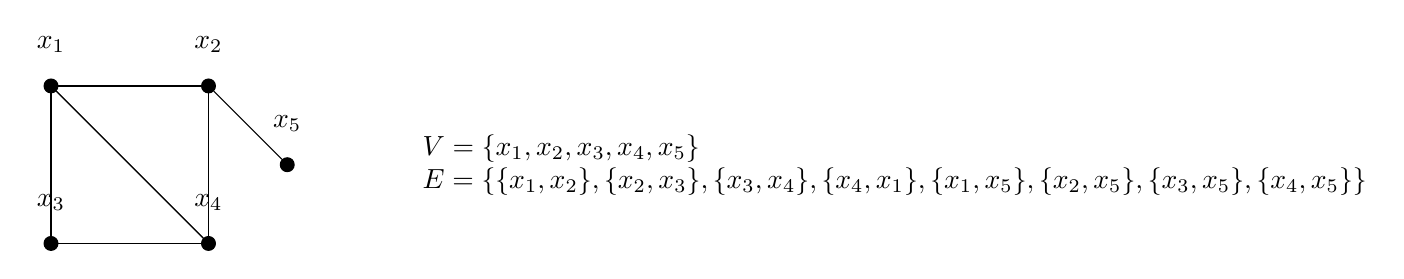
\begin{tikzpicture}
  % 定义点
  \node[circle,draw,fill=black,label=above:$x_1$,minimum size=5pt,inner sep=0pt] (x1) at (0,0) {};
  \node[circle,draw,fill=black,label=above:$x_2$,minimum size=5pt,inner sep=0pt] (x2) at (2,0) {};
  \node[circle,draw,fill=black,label=above:$x_3$,minimum size=5pt,inner sep=0pt] (x3) at (0,-2) {};
  \node[circle,draw,fill=black,label=above:$x_4$,minimum size=5pt,inner sep=0pt] (x4) at (2,-2) {};
  \node[circle,draw,fill=black,label=above:$x_5$,minimum size=5pt,inner sep=0pt] (x5) at (3,-1) {};

  % 定义边
  \draw (x1) -- (x2);
  \draw (x2) -- (x4);
  \draw (x1) -- (x3);
  \draw (x3) -- (x4);
  \draw (x1) -- (x4);
  \draw (x4) -- (x1);
  \draw (x2) -- (x5);

  \node[align=left, right=of x5, xshift=5mm]{
    $V = \{x_1, x_2, x_3, x_4, x_5\}$ \\
    $E = \{\{x_1, x_2\}, \{x_2, x_3\}, \{x_3, x_4\}, \{x_4, x_1\}, \{x_1, x_5\}, \{x_2, x_5\}, \{x_3, x_5\}, \{x_4, x_5\}\}$
  };
\end{tikzpicture}


$V$ is the \uline{\textcolor{MarkerColour}{\textsc{Vertex set}}} and $E$ is the \uline{\textcolor{MarkerColour}{\textsc{edge set}}}. We may also write $V(G)$ and $E(G)$ for $V$ and $E$. $|V|$ and $|E|$ are the \uline{\textcolor{MarkerColour}{\textsc{order}}} and \uline{\textcolor{MarkerColour}{\textsc{size}}} of $G$.

Note: No loops.

No multi edges.

\paragraph{Important examples:}

The \uline{\textcolor{MarkerColour}{\textsc{empty graph}}} $E_n$ of order $n$:

\begin{tikzpicture}
  % 定义点
  \node[circle,draw,fill=black,label=above:$x_1$,minimum size=5pt,inner sep=0pt] (x1) at (0,0) {};
  \node[circle,draw,fill=black,label=above:$x_2$,minimum size=5pt,inner sep=0pt] (x2) at (2,0) {};
  \node[circle,draw,fill=black,label=above:$x_3$,minimum size=5pt,inner sep=0pt] (x3) at (0,-2) {};
  \node[circle,draw,fill=black,label=above:$x_n$,minimum size=5pt,inner sep=0pt] (xn) at (2,-2){};

  \node[align=left, right=of x5, xshift=20mm]{
    $V = \{x_1, \cdots , x_n\}$
  };
\end{tikzpicture}

The \uline{\textcolor{MarkerColour}{\textsc{complete graph}}} $K_n$ of order n:

\begin{tikzpicture}
  % 定义样式
  \tikzset{vertex/.style = {circle, draw, fill=black, minimum size=5pt, inner sep=0pt}}
  \tikzset{edge/.style = {draw, thick}}

  % 定义点
  \node[vertex, label=above:$x_1$] (x1) at (0,0) {};
  \node[vertex, label=above:$x_2$] (x2) at (2,0) {};
  \node[vertex, label=below:$x_n$] (x3) at (2,-2) {};
  \node[vertex, label=below:] (x4) at (0,-2) {};

  % 定义边
  \draw[edge] (x1) -- (x2);
  \draw[edge] (x1) -- (x3);
  \draw[edge] (x1) -- (x4);
  \draw[edge] (x2) -- (x3);
  \draw[edge] (x2) -- (x4);
  \draw[edge] (x3) -- (x4);

  \node[align=left, right=of x3, xshift=20mm]{
    $V = \{x_1, \cdots,  x_5\}$, \ $E = \{x_ix_j\mid 1\leqslant i<j\leqslant n \}$ \\
    $|V| = n$,\ $|E| =\binom{n}{2}$
  };
\end{tikzpicture}

The \uline{\textcolor{MarkerColour}{\textsc{path}}} $P_n$ of order $n$, \uline{\textcolor{MarkerColour}{\textsc{length}}} $n-1$:

\usetikzlibrary{positioning, shapes.misc}
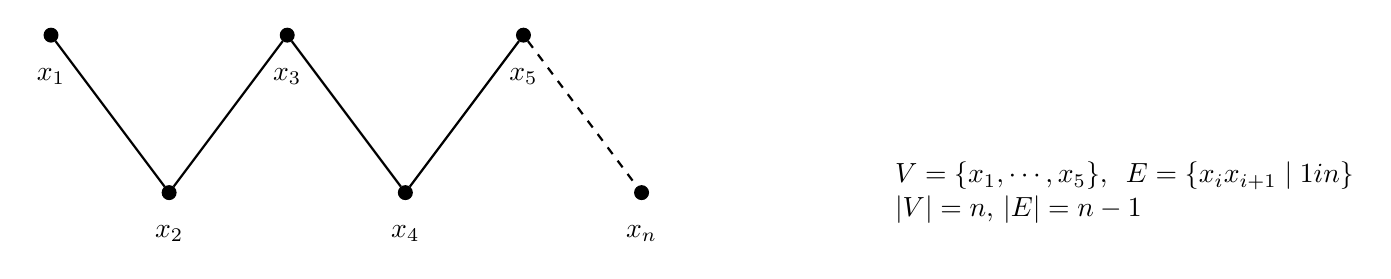
\begin{tikzpicture}
  % 定义样式
  \tikzset{vertex/.style = {circle, draw, fill=black, minimum size=5pt, inner sep=0pt}}
  \tikzset{edge/.style = {draw, thick}}
  \tikzset{dots/.style = {draw, thick, dashed}}

  % 定义点
  \node[vertex, label=below:$x_1$] (x1) at (0,1) {};
  \node[vertex, label=below:$x_2$] (x2) at (1.5,-1) {};
  \node[vertex, label=below:$x_3$] (x3) at (3,1) {};
  \node[vertex, label=below:$x_4$] (x4) at (4.5,-1) {};
  \node[vertex, label=below:$x_5$] (x5) at (6,1) {};
  \node[vertex, label=below:$x_n$] (xn) at (7.5,-1) {}; % Assuming x_n is x_6

  % 定义边
  \draw[edge] (x1) -- (x2);
  \draw[edge] (x2) -- (x3);
  \draw[edge] (x3) -- (x4);
  \draw[edge] (x4) -- (x5);
  \draw[dots] (x5) -- (xn); % Dashed line for ellipsis
    
    \node[align=left, right=of xn, xshift=20mm]{
    $V = \{x_1, \cdots,  x_5\}$, \ $E = \{x_ix_{i+1}\mid 1\leqslant i\leqslant n \}$ \\
    $|V| = n$,\ $|E| =n-1$
  };
\end{tikzpicture}

We may write $P_n = x_1x_2\cdots x_n$. We say that $x_1, x_n$ are the \uline{\textcolor{MarkerColour}{\textsc{end-vertices}}} of $P_n$, and $P_n$ is an \uline{\textcolor{MarkerColour}{\textsc{$x_1-x_n$ Path}}}.

The \uline{\textcolor{MarkerColour}{\textsc{cycle}}} $C_n$ of order and length $n\geqslant 3$: 
\usetikzlibrary{shapes.geometric, positioning, decorations.markings}

\begin{tikzpicture}
  % 定义半径和中心点
  \def\radius{1.5cm} % 半径为2cm
  \def\center{0,0} % 中心点为原点

  % 使用极坐标定义六边形的六个顶点
  \foreach \x/\angle in {1/0, 2/60, 3/120, 4/180, 5/240, n/300}
    \node[fill, circle, inner sep=2pt, label={[font=\small]\angle:$x_{\x}$}] (x\x) at ([shift={(\angle:\radius)}]\center) {};

  % 连接顶点
  \draw (x1) -- (x2) -- (x3) -- (x4) -- (x5) -- (xn) -- (x1) -- cycle;

  \node[align=left, right=of x1, xshift=20mm]{
    $V = \{x_1, \cdots,  x_n\}$, \ $E = \{x_ix_{i+1}\mid 1\leqslant i\leqslant n \}\cup\{x_nx_1\}$ \\
    $|V| = n$,\ $|E| =n$
  };
\end{tikzpicture}

We may write $C_n = x_1x_2\cdots x_nx_1$.

The \uline{\textcolor{MarkerColour}{\textsc{complete bipartite graph}}} $K_{m, n}$:

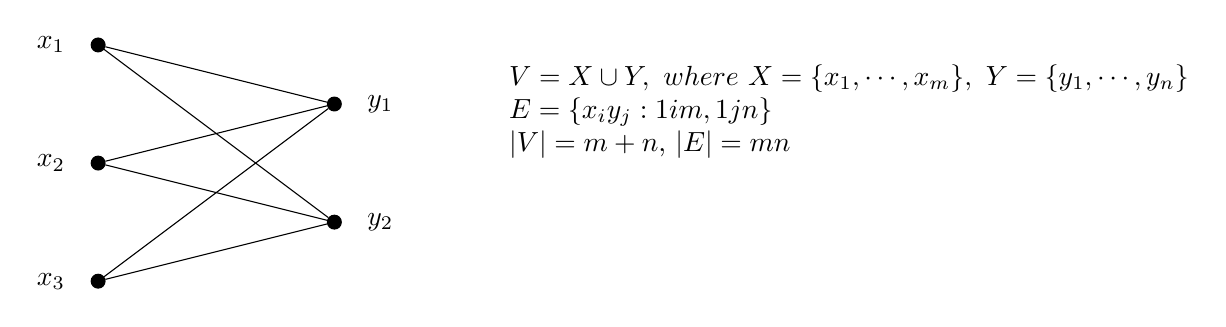
\begin{tikzpicture}[scale=1.5, vertex/.style={circle, draw, fill=black, minimum size=5pt, inner sep=0pt}]

  % 定义左侧顶点
  \node[vertex, label=left:$x_1$] (x1) at (0,2) {};
  \node[vertex, label=left:$x_2$] (x2) at (0,1) {};
  \node[vertex, label=left:$x_3$] (x3) at (0,0) {};

  % 定义右侧顶点
  \node[vertex, label=right:$y_1$] (y1) at (2,1.5) {};
  \node[vertex, label=right:$y_2$] (y2) at (2,0.5) {};

  % 绘制边连接顶点
  \foreach \i in {1,2,3}
    \foreach \j in {1,2}
      \draw (x\i) -- (y\j);

    \node[align=left, right=of y1, xshift=10mm, yshift=-1mm]{
    $V = X\cup Y,\ \text{where}\ X = \{x_1, \cdots, x_m\},\ Y = \{y_1, \cdots, y_n\}$ \\
    $E = \{x_iy_j:1\leqslant i\leqslant m, 1\leqslant j\leqslant n\}$ \\
    $|V| = m+n$, $|E| = mn$
  };
\end{tikzpicture}

In general, a graph $G = (V, E)$ is \uline{\textcolor{MarkerColour}{\textsc{bipartite}}} if we have $V = X\cup Y$ s.t. $E\subset \{xy\mid x\in X, y\in Y\}$.

$G^{\prime} = (V^{\prime}, E^{\prime})$ is a \uline{\textcolor{MarkerColour}{\textsc{subgraph}}} of $G = (V, E)$, written $G^{\prime}\subset G$, if $V^{\prime}\subset V$ and $E^{\prime}\subset E$. If $V^{\prime} = V$ and $E^{\prime}\subset E$, then $G^{\prime}$ is a \uline{\textcolor{MarkerColour}{\textsc{spanning subgraph}}} of $G$.

Let $G = (V, E)$. If $xy\in E$, then $x$ and $y$ are \uline{\textcolor{MarkerColour}{\textsc{neighbours}}} or \uline{\textcolor{MarkerColour}{\textsc{adjacent}}}. The \uline{\textcolor{MarkerColour}{\textsc{neighbourhood}}} of $x\in V$ is $\Gamma(x)$ (or $N(x)$) $=\{y\in V\mid xy\in E\}$. The \uline{\textcolor{MarkerColour}{\textsc{degree}}} of $x$ is $d(x) = |\Gamma(x)|$.

\begin{definition}[Directed Graph]
    A \uline{\textcolor{MarkerColour}{\textsc{directed graph}}} or \uline{\textcolor{MarkerColour}{\textsc{digraph}}} is a pair $D = (V, A)$, where $V$ is a set and $A$ is a set of ordered pairs from $V$.
\end{definition}

For example:

\usetikzlibrary{decorations.markings}
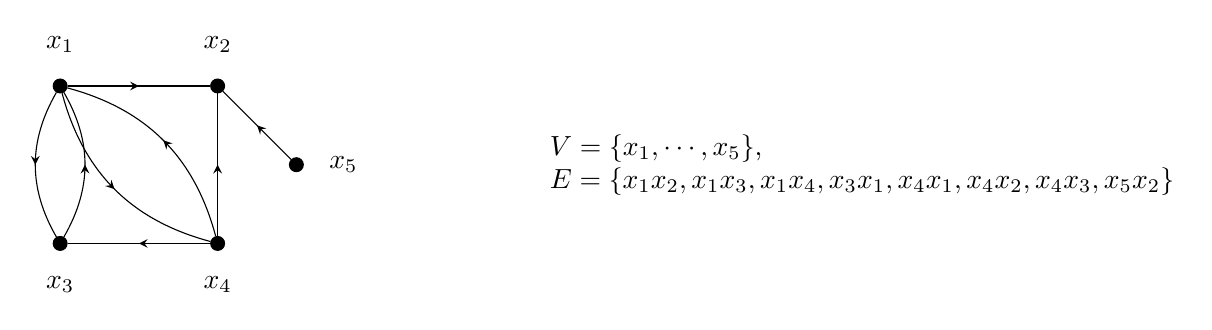
\begin{tikzpicture}[arrow1/.style={postaction={decorate}, decoration={
        markings,
        mark=at position 0.5 with {\arrow{stealth}} % 在中间位置添加箭头
    }},
    vertex/.style={circle, draw, fill=black, minimum size=5pt, inner sep=0pt}
]

  % 节点样式定义
  \tikzstyle{vertex} = [circle, draw, fill=black, minimum size=5pt, inner sep=0pt]

  % 定义节点
  \node[vertex, label=above:$x_1$] (x1) at (0,0) {};
  \node[vertex, label=above:$x_2$] (x2) at (2,0) {};
  \node[vertex, label=below:$x_3$] (x3) at (0,-2) {};
  \node[vertex, label=below:$x_4$] (x4) at (2,-2) {};
  \node[vertex, label=right:$x_5$] (x5) at (3,-1) {};

  % 绘制有向边
  \draw[arrow1] (x1) -- (x2);
  \draw[arrow1] (x4) -- (x2);
  \draw[arrow1] (x5) -- (x2);
  \draw[arrow1] (x4) -- (x3);

  % 绘制弧线
  \draw[arrow1, bend right] (x1) to (x3);
  \draw[arrow1, bend right] (x3) to (x1);
  \draw[arrow1, bend right] (x1) to (x4);
  \draw[arrow1, bend right] (x4) to (x1);

  % 绘制更复杂的弧线,比如回环
  % \draw[->, loop above] (x2) to (x2);
  \node[align=left, right=of x5, xshift=20mm]{
    $V = \{x_1, \cdots,  x_5\}$,\\
    $E = \{x_1x_2, x_1x_3, x_1x_4, x_3x_1, x_4x_1, x_4x_2, x_4x_3, x_5x_2 \}$
  };
\end{tikzpicture}

$V$ is the \uline{\textcolor{MarkerColour}{\textsc{vertex set}}}, and $A$ is the \uline{\textcolor{MarkerColour}{\textsc{arc set}}}. We may also write $V(D)$ and $A(D)$ for $V$ and $A$. $|V|$ and $|A|$ are the \uline{\textcolor{MarkerColour}{\textsc{order}}} and \uline{\textcolor{MarkerColour}{\textsc{size}}} of $D$.

Note: No loops.

No multiple arcs. But $x1-x2, x2-x1$ is acceptable.

\begin{example}
    The \uline{\textcolor{MarkerColour}{\textsc{complete diagraph}}} $K_n$ of order $n$:

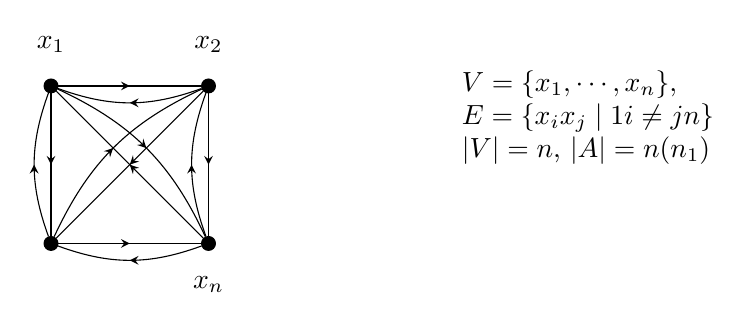
\begin{tikzpicture}[
    arrow in middle/.style={postaction={decorate}, decoration={
        markings,
        mark=at position 0.5 with {\arrow{stealth}}
    }},
    vertex/.style={circle, draw, fill=black, minimum size=5pt, inner sep=0pt}
]

  % 定义顶点位置
  \node[vertex, label=above:$x_1$] (x1) at (0,2) {};
  \node[vertex, label=above:$x_2$] (x2) at (2,2) {};
  \node[vertex, label=below:] (x3) at (0,0) {};
  \node[vertex, label=below:$x_n$] (x4) at (2,0) {};

  % 绘制有向边
  \foreach \from/\to in {x1/x2, x2/x3, x3/x4, x4/x1, x1/x3, x2/x4}
    \draw[arrow in middle] (\from) -- (\to);
  \foreach \from/\to in {x2/x1, x3/x2, x4/x3, x1/x4, x3/x1, x4/x2}
    \draw[arrow in middle, bend left=20] (\from) to (\to);

    \node[align=left, right=of x2, xshift=20mm, yshift = -4mm]{
    $V = \{x_1, \cdots,  x_n\}$,\\
    $E = \{x_ix_j\mid 1\leqslant i \neq j \leqslant n\}$ \\
    $|V| = n$, $|A| = n(n_1)$
  };
\end{tikzpicture}
\end{example}

\begin{example}
    The \uline{\textcolor{MarkerColour}{\textsc{directed path}}}, or \uline{\textcolor{MarkerColour}{\textsc{path}}} $\hat{P}_n$ of order $n$, length $n-1$:

    \vspace{0.5cm}
    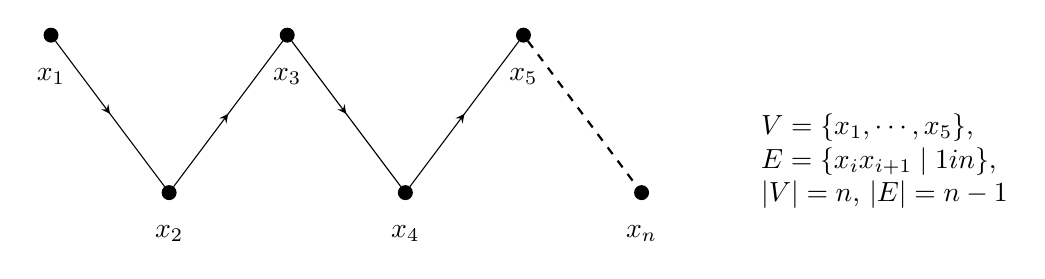
\begin{tikzpicture}[
    arrow in middle/.style={postaction={decorate}, decoration={
        markings,
        mark=at position 0.5 with {\arrow{stealth}}
    }},
    vertex/.style={circle, draw, fill=black, minimum size=5pt, inner sep=0pt}
]
  % 定义样式
  \tikzset{vertex/.style = {circle, draw, fill=black, minimum size=5pt, inner sep=0pt}}
  \tikzset{edge/.style = {draw, thick}}
  \tikzset{dots/.style = {draw, thick, dashed}}

  % 定义点
  \node[vertex, label=below:$x_1$] (x1) at (0,1) {};
  \node[vertex, label=below:$x_2$] (x2) at (1.5,-1) {};
  \node[vertex, label=below:$x_3$] (x3) at (3,1) {};
  \node[vertex, label=below:$x_4$] (x4) at (4.5,-1) {};
  \node[vertex, label=below:$x_5$] (x5) at (6,1) {};
  \node[vertex, label=below:$x_n$] (xn) at (7.5,-1) {}; % Assuming x_n is x_6

  % 定义边
  \draw[arrow in middle] (x1) -- (x2);
  \draw[arrow in middle] (x2) -- (x3);
  \draw[arrow in middle] (x3) -- (x4);
  \draw[arrow in middle] (x4) -- (x5);
  \draw[dots] (x5) -- (xn); % Dashed line for ellipsis
    
    \node[align=left, right=of xn, xshift=3mm, yshift = 4mm]{
    $V = \{x_1, \cdots,  x_5\}$, \\
    $E = \{x_ix_{i+1}\mid 1\leqslant i\leqslant n \}$, \\
    $|V| = n$,\ $|E| =n-1$
  };
\end{tikzpicture}

We may write $\hat{P}_n = x_1x_2\cdots x_n$. We say that $x_1, x_n$ are the \uline{\textcolor{MarkerColour}{\textsc{source}}} and \uline{\textcolor{MarkerColour}{\textsc{sink}}} of $\hat{P}_n$, and $\hat{P}_n$ is an $x_1 - x_n$ Path.
\end{example}

\begin{example}
    The \uline{\textcolor{MarkerColour}{\textsc{directed cycle}}}, or \uline{\textcolor{MarkerColour}{\textsc{dicycle}}} $\hat{C}_n$ of order and length $n\geqslant 3$ (Sometimes $n=2$ are allowed).

    \begin{tikzpicture}[
    arrow in middle/.style={postaction={decorate}, decoration={
        markings,
        mark=at position 0.5 with {\arrow{stealth}}
    }},
    vertex/.style={circle, draw, fill=black, minimum size=5pt, inner sep=0pt}
]
  % 定义半径和中心点
  \def\radius{1.5cm} % 半径为2cm
  \def\center{0,0} % 中心点为原点

  % 使用极坐标定义六边形的六个顶点
  \foreach \x/\angle in {1/0, 2/60, 3/120, 4/180, 5/240, n/300}
    \node[fill, circle, inner sep=2pt, label={[font=\small]\angle:$x_{\x}$}] (x\x) at ([shift={(\angle:\radius)}]\center) {};

  % 连接顶点
  \draw[arrow in middle] (x1) -- (x2) -- (x3) -- (x4) -- (x5) -- (xn) -- (x1);

  \node[align=left, right=of x1, xshift=20mm]{
    $V = \{x_1, \cdots,  x_n\}$, \ $E = \{x_ix_{i+1}\mid 1\leqslant i\leqslant n \}\cup\{x_nx_1\}$ \\
    $|V| = n$,\ $|E| =n$
  };
\end{tikzpicture}

We may write $\hat{C}_n = x_1x_2\cdots x_nx_1$. 
\end{example}

$D^{\prime} = (V^{\prime}, A^{\prime})$ is a \uline{\textcolor{MarkerColour}{\textsc{subdigraph}}} of $D = (V, A)$, written $D^{\prime}\subset D$, if $V^{\prime}\subset V$ and $A^{\prime} \subset A$. If $V^{\prime} = V$ and $A^{\prime}\subset A$, then $D^{\prime}$ is a \uline{\textcolor{MarkerColour}{\textsc{spanning subdigraph}}} of $D$.

Let $D = (V, A)$. If $xy\in A$, then $Y$ is an \uline{\textcolor{MarkerColour}{\textsc{out-neighbour}}} of $x$ and $x$ is an \uline{\textcolor{MarkerColour}{\textsc{in-neighbour}}} of $y$. The \uline{\textcolor{MarkerColour}{\textsc{out-neighbourhood/in-neighbourhood}}} of $x\in V$ are $\Gamma^{+}(x) = \{y\in V: xy\in A\}$ and $\Gamma^{-}(x) = \{y\in V: yx\in A\}$. The \uline{\textcolor{MarkerColour}{\textsc{out-degree/in-degree}}} of $x\in V$ are $d^+(x) = |\Gamma^+(x)|$ and $d^-(x) = |\Gamma^-(x)|$.

For a digraph $D = (V, A)$, the \uline{\textcolor{MarkerColour}{\textsc{underlying graph}}} is $G = (V, E)$ where $E = \{xy\mid xy\in A\ or\ yx\in A\}$.

A graph $G = (V, E)$ is \uline{\textcolor{MarkerColour}{\textsc{connected}}} if $\forall x, y\in V$, $\exists x-y$ path $P\subset G$. A digraph $D = (V, A)$ is \uline{\textcolor{MarkerColour}{\textsc{connected}}} if the underlying graph of $D$ is connected, and \uline{\textcolor{MarkerColour}{\textsc{strong-connected}}} if $\forall x, y\in V$, $\exists x-y$ path $\hat{P}\subset D$.

\uline{\textcolor{MarkerColour}{\textsc{A network graph}}} is a pair $(G, w)$, where $G$ is a graph, and $w\mid E(G)\to\mathbb{R}$. A \uline{\textcolor{MarkerColour}{\textsc{network digraph}}} is a pair $(D, w)$, where $D$ is a digraph, and $w\mid A(D)\to\mathbb{R}$. In each case, $w$ is a \uline{\textcolor{MarkerColour}{\textsc{weight function}}}.

From now on, we assume $V$ is finite, $\forall$ graphs and digraphs. In many situations, we consider connected graphs and digraphs.

\section{Shortest path problem}
\begin{definition}
    Let $(D, w)$ be a network digraph and $x, y\in V(D)$. A \uline{\textcolor{MarkerColour}{\textsc{walk}}} from $x$ to $y$, or an \uline{\textcolor{MarkerColour}{\textsc{$x-y$ walk}}}, is a sequence vertices $x = v_0, v_1, \cdots, v_k = y$ s.t. $v_{i-1}v_i\in A(D)$, $\forall 1\leqslant i\leqslant k$. Note that $v_0, v_1, \cdots, v_k$ and $v_0 v_1 \cdots v_{k-1} v_k$ are not necessarily distinct.
\end{definition}

\vspace{0.5cm}
\begin{tikzpicture}[
    arrow in middle/.style={postaction={decorate}, decoration={
        markings,
        mark=at position 0.5 with {\arrow{stealth}}
    }},
    vertex/.style={circle, draw, fill=black, minimum size=5pt, inner sep=0pt}
]
  % 定义样式
  \tikzset{vertex/.style = {circle, draw, fill=black, minimum size=5pt, inner sep=0pt}}
  \tikzset{edge/.style = {draw, thick}}
  \tikzset{dots/.style = {draw, thick, dashed}}

    \node[vertex, label=left:$x_1$](x1) at (0, 0) {};
    \node[vertex, label=below:](x2) at (1, 0) {};
    \node[vertex, label=below:](x3) at (2, 0) {};
    \node[vertex, label=below:](x4) at (3, 0) {};
    \node[vertex, label=below:](x5) at (4, 0) {};
    \node[vertex, label=below:$y$](x6) at (8, 0) {};
    \node[vertex, label=below:](x7) at (4, 2) {};
    \node[vertex, label=below:](x8) at (6, 2) {};
    \node[vertex, label=below:](x9) at (8, 2) {};

    \draw[arrow in middle] (x1) -- (x2) -- (x3) -- (x4) -- (x5) -- (x6);
    \draw[arrow in middle] (x5) to[out=90, in=180] (x7)
                               to[out=0, in=180] (x8)
                               to[out=0, in=180] (x9)
                               to[out=0, in=90] (x6);
\end{tikzpicture}

We say that $y$ is \uline{\textcolor{MarkerColour}{\textsc{reachable}}} from $x$ if $\exists$ an $x-y$ walk (equivalently, $\exists x-y$ path) in $D$. In this case, a \uline{\textcolor{MarkerColour}{\textsc{shortest path}}} from $x$ to $y$ is an $x-y$ walk. $x = v_0,v_1,\cdots, v_k =y$ with minimum weight, that is, $\sum\limits_{i=1}^k w(v_{i-1}, v_i)$ is minimum. Note that $D$ is strong connected $\Longleftrightarrow$ \ $y$ is reachable from $x$, $\forall\ x, y\i V(D)$.

We consider the following problem.
\subsection{Problem 3.1 Shortest path problem}
Let $(D, w)$ be a network digraph. Let $x\in V(D)$ s.t. $\forall \ y\in V(D)\backslash \{x\}$, $y$ is reachable from $x$. Find a shortest path from $x$ to every $y\in V(D)\backslash \{x\}$. We call $x$ the \uline{\textcolor{MarkerColour}{\textsc{source vertex}}}.

We consider two algorithms for solving Problem 3.1.
\subsubsection{A. Dijkstra's Algorithm}
We assume $w: A(D)\to \mathbb{R}_{\geqslant 0}$ in Problem 3.1. As Dijkstra's Algorithm is performed, every vertex $y\in V(D)$ is given a temporary label $T(y)$ which gets updated, then eventually a permanent label $P(y)$, which will be the weight of a shortest path from $x$ to $y$. Then algorithm is as follows.

\paragraph{1.} Set $P(x) = 0$, and
\begin{align*}
    T(y) = \left\lbrace\begin{array}{ll}
        w(xy), &\ \text{if} \ y\in \Gamma^+(x)  \\
        \infty, &\ \text{if} \ y\in V(D)\backslash \{\Gamma^+(x)\cup\{x\}\}
    \end{array} \right.
\end{align*}

Then, choose $y\in\Gamma^+(x)$ with $T(y)$ minimum, and set $P(y) = T(y)$.

\paragraph{2} Now, suppose $z\in V(D)$ is the most recent vertex to receive a permanent label, that is, to have $P(z)$ defined. $\forall v\in \Gamma^+(z)$ s.t. $T(v)$ but not $P(v)$ is defined, update
\begin{align*}
    T(v) = \min\left( T(v), P(z) + w(zv)\right)
\end{align*}

Then $\forall u\in V(D)$ s.t. $T(u)$ but not $P(u)$ is defined, choose $y$ where $T(y)$ is minimum, and set $P(y) = T(y)$. 

\paragraph{3} Return to Step $2$. Repeat procedure until termination.

\begin{remark}
    \begin{itemize}
        \item In Step 1 and 2 if there is a tie for the minimum, we may not choose any such suitable $y$.
        \item The assumption $w: A(D) \to \mathbb{R}_{\geqslant 0}$ implies that any shortest path from $x$ is in fact a path.
    \end{itemize}
\end{remark}

\setcounter{example}{0}
\begin{example}
    Find the shortest paths from $x_1$ to all other vertices, where $(D, w)$ is:
    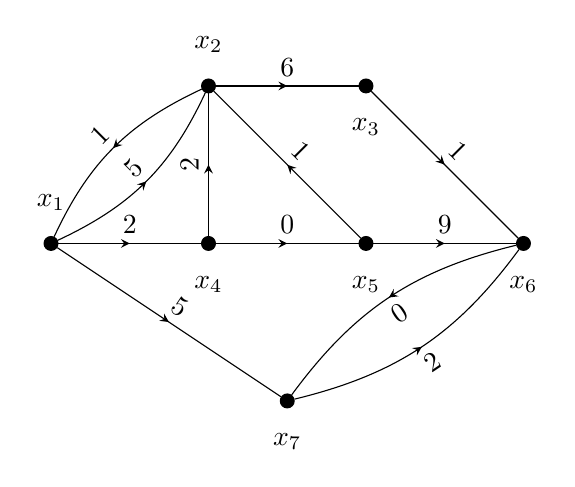
\begin{tikzpicture}[
    arrow in middle/.style={postaction={decorate}, decoration={
        markings,
        mark=at position 0.5 with {\arrow{stealth}}
    }},
    vertex/.style={circle, draw, fill=black, minimum size=5pt, inner sep=0pt}
]

  % 定义顶点位置
  \node[vertex, label=above:$x_1$] (x1) at (0,0) {};
  \node[vertex, label=above:$x_2$] (x2) at (2,2) {};
  \node[vertex, label=below:$x_3$] (x3) at (4,2) {};
  \node[vertex, label=below:$x_4$] (x4) at (2,0) {};
  \node[vertex, label=below:$x_5$] (x5) at (4,0) {};
  \node[vertex, label=below:$x_6$] (x6) at (6,0) {};
  \node[vertex, label=below:$x_7$] (x7) at (3,-2) {};
    
  % 绘制有向边并添加数字标签
  \draw[arrow in middle] (x1) to [bend right=20] node[midway, above, sloped] {5} (x2);
  \draw[arrow in middle] (x2) to [bend right=20] node[midway, above, sloped] {1} (x1);

  % 其他连线,如果需要标注也可以添加
  \draw[arrow in middle] (x6) to [bend right=20] node[midway, below, sloped] {0} (x7);
  \draw[arrow in middle] (x7) to [bend right=20] node[midway, below, sloped] {2} (x6);  % 替换“标签”为实际数值

  \draw[arrow in middle] (x1) -- (x4) node[midway, above, sloped] {2};
  \draw[arrow in middle] (x4) -- (x5) node[midway, above, sloped] {0};
  \draw[arrow in middle] (x5) -- (x6) node[midway, above, sloped] {9};
  \draw[arrow in middle] (x4) -- (x2) node[midway, above, sloped] {2};
  \draw[arrow in middle] (x5) -- (x2) node[midway, above, sloped] {1};

  \draw[arrow in middle] (x2) -- (x3) node[midway, above, sloped] {6};
  \draw[arrow in middle] (x1) -- (x7) node[midway, above, sloped] {5};
  \draw[arrow in middle] (x3) -- (x6) node[midway, above, sloped] {1};
  %\draw[arrow in middle] (x4) -- (x2) node[midway, above, sloped] {2};
  
\end{tikzpicture}
\end{example}

We initially set 
\begin{table}[H]
    \centering
    \begin{tabular}{|ccccccc|}
    \hline
       $x_1$ & $x_2$ & $x_3$ & $x_4$ & $x_5$ & $x_6$ & $x_7$   \\ \hline
    \uline{$0^*$} & 5 & $\infty$ & $2^{\boxed{*}}$ & $\infty$ & $\infty$ & 5 \\ \hline
    \end{tabular}
\end{table}
where $\_$ means the out-neighbour of this vertex (z in Step 2) are being considered, and ${}^*$ is a permanent label, with $^{\boxed{*}}$ the newest one. The next iteration is 
\begin{table}[H]
    \centering
    \begin{tabular}{|ccccccc|}
    \hline
       $x_1$ & $x_2$ & $x_3$ & $x_4$ & $x_5$ & $x_6$ & $x_7$   \\ \hline
    $0^*$ & 4 & $\infty$ & \uline{$2^*$} & $2^{\boxed{*}}$ & $\infty$ & 5 \\ \hline
    \end{tabular}
\end{table}

New temporary labels:
\begin{align*}
    x_2: & \min(5, 2+2) = 4\\
    x_5: & \min(\infty, 2+0) = 2
\end{align*}

$2 = \min(4, 2, 5)$, this becomes permanent.

Repeating, we obtain:
\begin{table}[H]
    \centering
    \begin{tabular}{|ccccccc|}
    \hline
       $x_1$ & $x_2$ & $x_3$ & $x_4$ & $x_5$ & $x_6$ & $x_7$   \\ \hline
    $0^*$ & $3^{\boxed{*}}$ & $\infty$ & $2^*$ & \uline{$2^*$} & $5$ & 5 \\
    $0^*$ & \uline{$3^*$} & $9$ & $2^*$ & $2^*$ & $5^{\boxed{*}}$ & 5 \\
    $0^*$ & $3^*$ & $9$ & $2^*$ & $2^*$ & \uline{$5^*$} & $5^{\boxed{*}}$ \\
    $0^*$ & $3^*$ & $9^{\boxed{*}}$ & $2^*$ & $2^*$ & $5^*$ & \uline{$5^{*}$} \\
    \hline
    \end{tabular}
\end{table}

We obtain a \uline{shortest paths tree from $x_1$ as}:

\begin{tikzpicture}[
    arrow in middle/.style={postaction={decorate}, decoration={
        markings,
        mark=at position 0.5 with {\arrow{stealth}}
    }},
    vertex/.style={circle, draw, fill=black, minimum size=5pt, inner sep=0pt}
]

  % 定义顶点位置
  \node[vertex, label=above:$x_1$] (x1) at (0,0) {};
  \node[vertex, label=above:$x_2$] (x2) at (2,2) {};
  \node[vertex, label=below:$x_3$] (x3) at (4,2) {};
  \node[vertex, label=below:$x_4$] (x4) at (2,0) {};
  \node[vertex, label=below:$x_5$] (x5) at (4,0) {};
  \node[vertex, label=below:$x_6$] (x6) at (6,0) {};
  \node[vertex, label=below:$x_7$] (x7) at (3,-2) {};
  
  \draw[arrow in middle] (x1) -- (x4) node[midway, above, sloped] {2};
  \draw[arrow in middle] (x4) -- (x5) node[midway, above, sloped] {0};
  \draw[arrow in middle] (x5) -- (x6) node[midway, above, sloped] {9};
  % \draw[arrow in middle] (x4) -- (x2) node[midway, above, sloped] {2};
  \draw[arrow in middle] (x5) -- (x2) node[midway, above, sloped] {1};

  \draw[arrow in middle] (x2) -- (x3) node[midway, above, sloped] {6};
  \draw[arrow in middle] (x1) -- (x7) node[midway, above, sloped] {5};
  % \draw[arrow in middle] (x3) -- (x6) node[midway, above, sloped] {1};
  % \draw[arrow in middle] (x4) -- (x2) node[midway, above, sloped] {2};
  
\end{tikzpicture}

To obtain a shortest path from $x_1$ to $y$, look at when $y$ is given ${}^{\boxed{*}}$, and backtrack.

\begin{theorem}
    Let $(D, w)$ be a network digraph, where $w:A(D)\to\mathbb{R}_{\geqslant 0}$. Then Dijkstra's Algorithm solves Problem 3.1.
\end{theorem}
\begin{proof}
    Let $R_t\subset V(D)$ be the set of permanently labelled vertices after $t$ iterations of Dijkstra's Algorithm. Note that $R_t = R_{t-1}\cup\{y\}$, where $y$ becomes permanently labelled at the $t^{th}$ iteration ($1<t\leqslant |V(D)|$). We use induction on $t$ to show that $P(z) = W(z)$, $\forall z\in R_t\backslash \{x\}$, where $W(z)$ is the weight of a shortest path from $x$ to $z$.

   \paragraph{Base cases:} $t=1: R_1=\{x\}, not \exists z\in R_1\backslash\{x\}$.

   $t = 2$: Let $R_2=\{x, z\}$. Then clearly, $w(xz) \leqslant$ weight of any $x-z$ walk since $w:A(D)\to \mathbb{R}_{\geqslant 0}$.

   \paragraph{Induction Step} Let $t\geqslant 3$, and suppose $P(z) = W(z)$, $\forall z\in R_{t-1}\backslash\{x\}$. Let $R_t = R\cup\{y\}$. We show that $P(y) = W(y)$. Clearly, $P(y)\geqslant W(y)$. Suppose that $P(y)>W(y)$. Let $v_0 v_1\cdots v_k$ be a shortest path from $x$ to $y$. $(v_0 = x, v_k = y)$ with $\sum\limits_{i=1}^k w(v_{i-1} v_i) = W(y)$. Since $y\in R_{t-1}$, $\exists 0\leqslant l\leqslant k$ s.t. $v_i\in R_{t-1}$, $\forall 0\leqslant i\leqslant l$, and $v_{l+1}\notin R_{t+1}$, then 
   \begin{align*}
       P(y) > \sum\limits_{i=1}^k w(v_{i-1}v_i) \geqslant \sum\limits_{i=1}^k w(v_{i-1}v_i) + w(v_l v_{l+1}) \geqslant P(v_l) + w(v_lv_{l+1}) \geqslant T(v_{l+1}) \geqslant P(y)
   \end{align*}
    where $T_(v_{l+1})$ is the temporary label of $v_{l+1}$ at the $t^{th}$ iteration. To see $(*)$, note that at some iteration before $t$, $v_l$ was given the permanent label $P(v_l)$, and $v_{l+1}$ was given a temporary label $\leqslant P(v_l) + w(v_l v_{l+1})$. $+$ holds since at $t^{th}$ iteration, $y$ is given a permanent label over $v_{l+1}$ or $y=v_{l+1}$.

    We have a contradiction. The induction step holds. The proof follows by letting $R_t = V(D)$.
\end{proof}

\subsubsection{Bellman-Fold Algorithm}
Now, let $w:A(D)\to \mathbb{R}$ in Problem 3.1, so arcs of $D$ may have negative weights. Then Dijkstra's Algorithm fails. A major problem is if $D$ has a \uline{negative dicycle} $\vec{C}=v_1 v_2\cdots v_k v_1\ (k\geqslant 2)$, where $\sum\limits_{i=1}^k w(v_i v_{i+1}) < 0\ (v_{k+1} = v_1)$. Then no shortest path exists from $x$ to any $v_i$, since we may reach $v_i$ from $x$, then go around $\vec{C}$ as much as we like. Dijkstra's Algorithm does not detect this problem, since at each iteration, only vertices without a permanent label are explored. Even if $D$ has no dicycle, there is still a problem like:

\tikzset{
    big arrow/.style={
        decoration={
            markings,
            mark=at position 0.5 with {\arrow[scale=2]{stealth}} % 调整这里的scale值来改变箭头大小
        },
        postaction={decorate}
    },
    vertex/.style={circle, draw, fill=black, minimum size=5pt, inner sep=0pt},
    label distance=2mm  % 调整标签距离线的距离
}

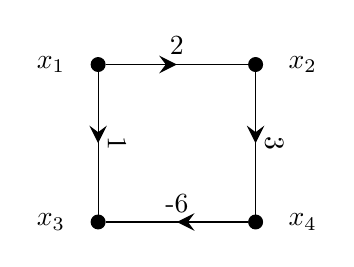
\begin{tikzpicture}[
    vertex/.style={circle, draw, fill=black, minimum size=5pt, inner sep=0pt},
    label distance=2mm  % 调整标签距离线的距离
]

  % 定义顶点位置
  \node[vertex, label=left:$x_1$] (x1) at (0,0) {};
  \node[vertex, label=right:$x_2$] (x2) at (2,0) {};
  \node[vertex, label=left:$x_3$] (x3) at (0,-2) {};
  \node[vertex, label=right:$x_4$] (x4) at (2, -2) {};

  % 绘制有向边并添加数字标签
  \draw[big arrow] (x1) -- (x2) node[midway, above, sloped] {2};
  \draw[big arrow] (x2) -- (x4) node[midway, above, sloped] {3};
  \draw[big arrow] (x4) -- (x3) node[midway, above, sloped] {-6};
  \draw[big arrow] (x1) -- (x3) node[midway, above, sloped] {1};

\end{tikzpicture}

If $x_1$ is the source vertex, then Dijkstra's Algorithm gives $P(x_3) = 1$. But the shortest path from $x_1$ to $x_3$ is $x_1x_2x_4x_3$, with weight $-1$. Then proof Th 3.2 breaks down at the base case $t=2$, and also at the induction step.

The \uline{\textcolor{MarkerColour}{\textsc{Bellman-Ford Algorithm}}} can overcome these problems, and detect the presence of a negative dicycle, but takes more work than Dijkstra's Algorithm. As we run the algorithm, each vertex $y\in V(D)$ has its label $L(y)$ updated, which is the currently known weight of an $x-y$ walk. The algorithm is as follows:

\paragraph{1}Fix an ordering of the arcs of $D$, say $a_1, \cdots, a_m$, where $m = |A(D)|$.

\paragraph{2}Set $L(x) = 0$ and $L(y) = \infty$, $\forall y\in V(D)\backslash\{x\}$.

\paragraph{3}In one round, we run through $a_1, \cdots, a_m$. When we consider $a_i = uv$ say, update $L(v)$ by
\begin{align*}
    L(v) = \min(L(v), L(u) + w(uv) )
\end{align*}

\paragraph{4}Repeat Step 3. If after $\leqslant |V(D)| - 1$ rounds, $L(y)$ does not decrease $\forall y\in V(D)$, then the resulting $L(y)$ are the weights of these shortest paths from $x$ to every $y\in V(D)\backslash\{x\}$. Otherwise, $\exists$ negative dicycle in $D$.

Note that:
\begin{itemize}
    \item After $r$ rounds step $3$, all walks from $x$ with $\leqslant r$ arcs are found.
    \item If at round $|V(D)|$, some $L(y)$ is updated, then an $x$-$y$ walk with $\geqslant |V(D)|$ arcs and weight $L(y)$ has been found. Such a walk contains a dicycle, and then can only exist if $D$ has a negative dicycle. 
\end{itemize}

\setcounter{example}{1}
\begin{example}
    Find the shortest paths from $x_1$ to all others vertices when $(D, w)$ is the following:
    \tikzset{
    big arrow/.style={
        decoration={
            markings,
            mark=at position 0.5 with {\arrow[scale=2]{stealth}} % 调整这里的scale值来改变箭头大小
        },
        postaction={decorate}
    },
    vertex/.style={circle, draw, fill=black, minimum size=5pt, inner sep=0pt},
    label distance=2mm  % 调整标签距离线的距离
}

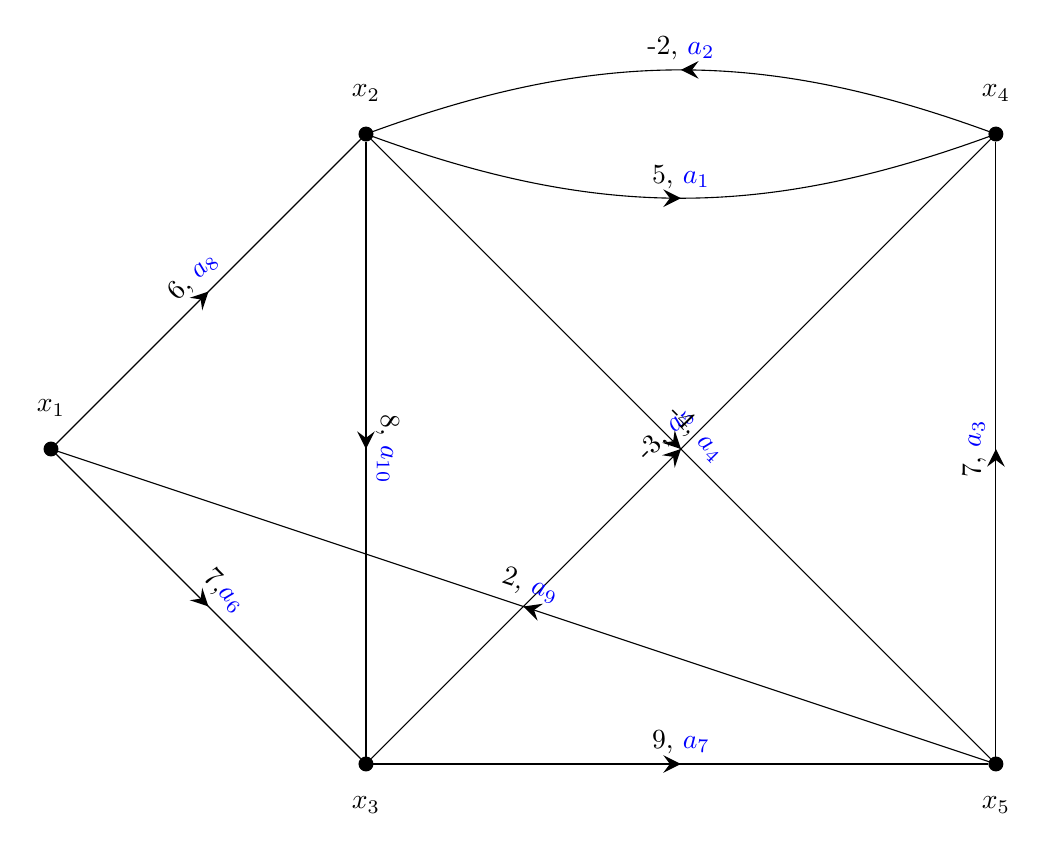
\begin{tikzpicture}[
    vertex/.style={circle, draw, fill=black, minimum size=5pt, inner sep=0pt},
    label distance=2mm  % 调整标签距离线的距离
]

  % 定义顶点位置
  \node[vertex, label=above:$x_2$] (x2) at (4,4) {};
  \node[vertex, label=below:$x_3$] (x3) at (4,-4) {};
  \node[vertex, label=above:$x_4$] (x4) at (12,4) {};
  \node[vertex, label=below:$x_5$] (x5) at (12, -4) {};
  \node[vertex, label=above:$x_1$] (x1) at (0, 0) {};

  % 绘制有向边并添加数字标签
  \draw[big arrow] (x1) -- (x2) node[midway, above, sloped] {6, \textcolor{blue}{$a_8$}};
  \draw[big arrow] (x1) -- (x3) node[midway, above, sloped] {7,\textcolor{blue}{$a_6$}};
  \draw[big arrow] (x3) -- (x4) node[midway, above, sloped] {-3, \textcolor{blue}{$a_5$}};
  \draw[big arrow] (x5) -- (x1) node[midway, above, sloped] {2, \textcolor{blue}{$a_9$}};
  \draw[big arrow] (x2) -- (x5) node[midway, above, sloped] {-4, \textcolor{blue}{$a_4$}};
  \draw[big arrow] (x5) -- (x4) node[midway, above, sloped] {7, \textcolor{blue}{$a_3$}};
  \draw[big arrow] (x3) -- (x5) node[midway, above, sloped] {9, \textcolor{blue}{$a_7$}};
  \draw[big arrow] (x2) -- (x3) node[midway, above, sloped] {8, \textcolor{blue}{$a_{10}$}};
  
  \draw[big arrow] (x2) to [bend right=20] node[midway, above, sloped] {5, \textcolor{blue}{$a_1$}} (x4);
  \draw[big arrow] (x4) to [bend right=20] node[midway, above, sloped] {-2, \textcolor{blue}{$a_2$}} (x2);
  
  
\end{tikzpicture}
\end{example}

Fix the arc ordering $a_1, \cdots, a_{10}$ as shown. In round 1, we have
\begin{table}[H]
    \centering
    \begin{tabular}{|c|ccccc|c}
        \cline{1-6}
         & $x_1$ & $x_2$ & $x_3$ & $x_4$ & $x_5$ & \\ \cline{1-6}
        Initially & 0 & $\infty$ &  $\infty$  &  $\infty$ &  $\infty$ & \\ 
        After $a_1, \cdots, a_6$ & \boxed{0} &  $\infty$  & \boxed{7} &  $\infty$  &  $\infty$ & \textcolor{blue}{$a_6$}\\
        After $a_7$ & 0 &  $\infty$  & 7 &  $\infty$  & 16 & \\
        After $a_8$ & 0 & 6 & 7 &  $\infty$ & 16 & \\
        After $a_9$, $a_{10}$ & 0 & 6 & 7 & $\infty$ & 16 & \\ \cline{1-6}
    \end{tabular}
    \caption{Round 1}
\end{table}

\begin{table}[H]
    \centering
    \begin{tabular}{|c|ccccc|c}
        \cline{1-6}
         & $x_1$ & $x_2$ & $x_3$ & $x_4$ & $x_5$ & \\ \cline{1-6}
        Initially & 0 & 6 & 7 & $\infty$ & 16  &  \\ 
        After $a_1$ & 0 & 6  & 7 & 11 & 16  & \\
        After $a_2, a_3, a_4$ & 0 & 6  & 7 & 11  & 2 & \\
        After $a_5$ & 0 & 6 & \boxed{7} &  \boxed{4} & 2 & \textcolor{blue}{$a_5$} \\
        After $a_6, \cdots, a_{10}$ & 0 & 6 & 7 & 4 & 2 &  \\ \cline{1-6}
    \end{tabular}
    \caption{Round 2}
\end{table}

\begin{table}[H]
    \centering
    \begin{tabular}{|c|ccccc|c}
        \cline{1-6}
         & $x_1$ & $x_2$ & $x_3$ & $x_4$ & $x_5$ & \\ \cline{1-6}
        Initially & 0 & 6 & 7 & 4 & 2   & \\ 
        After $a_1, a_2$ & 0 & \boxed{2}  & 7 & \boxed{4} & 2 & \textcolor{blue}{$a_2$} \\
        After $a_3, a_4$ & 0 & \boxed{2}  & 7 & 4  & \boxed{-2} &  \textcolor{blue}{$a_4$}\\
        After $a_5, \cdots, a_{10}$ & 0 & 2 & 7 & 4 & -2 & \\ \cline{1-6}
    \end{tabular}
    \caption{Round 3}
    \label{Round 3}
\end{table}

We can then show that round $4$ does not update the bottom row of \ref{Round 3}. The weights of the shortest paths from $x_1$, are given by the bottom row of \ref{Round 3}. We can easily backtrack to obtain the shortest paths tree from $x_1$.

\tikzset{
    big arrow/.style={
        decoration={
            markings,
            mark=at position 0.5 with {\arrow[scale=2]{stealth}} % 调整这里的scale值来改变箭头大小
        },
        postaction={decorate}
    },
    vertex/.style={circle, draw, fill=black, minimum size=5pt, inner sep=0pt},
    label distance=2mm  % 调整标签距离线的距离
}

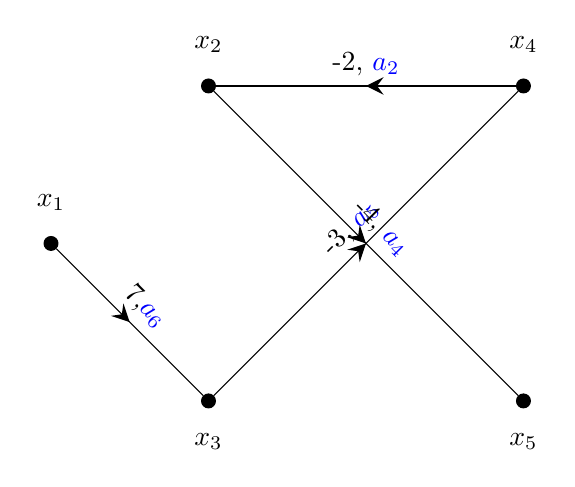
\begin{tikzpicture}[
    vertex/.style={circle, draw, fill=black, minimum size=5pt, inner sep=0pt},
    label distance=2mm  % 调整标签距离线的距离
]

  % 定义顶点位置
  \node[vertex, label=above:$x_2$] (x2) at (2,2) {};
  \node[vertex, label=below:$x_3$] (x3) at (2,-2) {};
  \node[vertex, label=above:$x_4$] (x4) at (6,2) {};
  \node[vertex, label=below:$x_5$] (x5) at (6, -2) {};
  \node[vertex, label=above:$x_1$] (x1) at (0, 0) {};

  % 绘制有向边并添加数字标签
  \draw[big arrow] (x4) -- (x2) node[midway, above, sloped] {-2, \textcolor{blue}{$a_2$}};
  \draw[big arrow] (x1) -- (x3) node[midway, above, sloped] {7,\textcolor{blue}{$a_6$}};
  \draw[big arrow] (x3) -- (x4) node[midway, above, sloped] {-3, \textcolor{blue}{$a_5$}};
  \draw[big arrow] (x2) -- (x5) node[midway, above, sloped] {-4, \textcolor{blue}{$a_4$}};
\end{tikzpicture}

For example, for $x_5$, see the circle entries. The shortest path has arcs $a_6$, $a_5$, $a_2$, $a_4$.

\begin{theorem}
    Let $(D, w)$ be a network digraph, where $w: A((D)\to R$. Suppose we apply the Bellman-Ford Algorithm to solve Problem 3.1.
    \begin{itemize}
        \item[\textbf{(a)}] Suppose for some $1\leqslant r\leqslant |V(D)|-1$, when going from round $r$ to round $r+1$, the algorithm does not update $L(y)$, $\forall y\in V(D)$. Then $L(y)$ after round $r$ is the weight of the shortest path from $x$ to $y$, $\forall y\in V(D)\backslash\{x\}$, and $L(x)=0$ at all times.
        \item[\textbf{(b)}] If when going from round $|V(D)|-1$ to $|V(D)|$, the algorithm updates $L(y)$ for some $y\in V(D)$, then $\exists$ negative dicycle $\vec{C}\subset D\ (|V(\vec{C}) \geqslant 2)$. Moreover, for $z\in V(D)\backslash \{x\}$, $\exists$ shortest path (with finite weight) from $x$ to $z\Longleftrightarrow\ z$ is not reachable from any vertex of a negative dicycle of $D$.
    \end{itemize} 
\end{theorem}

\begin{proof}
    \textbf{(a)} Note that no $L(y)$ is updated when we go from round $s$ to round $s+1$, $\forall s\geqslant r$. Suppose $\exists\ z\in V(D)\backslash\{x\}$, s.t. at round $s$, $\exists s\geqslant r$, we have $L(z)>W(z)$, where 
    \begin{align*}
        W(z) = \left\lbrace\begin{array}{ccc}
            \textrm{Minimum weight of an }x-z \textrm{ walk,} &\  \textrm{if finite}, & (1) \\
            -\infty, & \ \textrm{otherwise} & (2)
        \end{array} \right.
    \end{align*}

    If (1) holds, then $\exists$ x-z walk with weight $W(z)$, which is in fact an $x$-$z$ path $\vec{P}$ (see HW5), so $|A(\vec{P})| \leqslant |V(D)| - 1$. But then $\vec{P}$ would be realised by the algorithm at round $|V(D)| - 1$, when we have $L(z)\leqslant W(z) < L(z)$, a contradiction. 

    If (2) holds, then $\exists$ sequence of $x$-$z$ walks, whose weights strictly decrease and $\to - \infty$. By running the algorithm for as many rounds as we like, all these weights will be realised, and so $L(z)\to -\infty$, a contradiction.

    Finally, if $L(x)<0$ after some number of rounds, then $\exists$ negative dicycle containing $x$. Running the algorithm as long as we like, we have $L(x)\to -\infty$, a contradiction.

    \textbf{(b)} If $y=x$, then proof of last part of (a) $\Longrightarrow$ $\exists$ negative dicycle. Now let $y\neq x$. If $\exists v\in V(D)\backslash \{x\}$ s.t. $\neg\exists$ shortest path from $x$ to $v$. ($\forall M>0,\ \exists\ x-v $ walk with weight $\leqslant -M$), then $\exists$ negative dicycle (HW5). Otherwise, $\forall y\in V(D)\backslash\{x\}$, $\exists$ shortest path from $x$ to $y$, and this is an $x-y$ path(HW5), with $\leqslant |V(D)| - 1$ arcs. Hence, the algorithm cannot update after round $|V(D)| - 1$, a contradiction.

    Final part: $(\Longrightarrow)$ If $z$ is reachable from some vertex $u$ of a negative dicycle $\vec{C}$, then we may reach $u$ from $x$, go around $\vec{C}$ as much as we like, then reach $z$ from $u$. Then $\neg\exists$ shortest path from $x$ to $z$.

    $(\Longleftarrow)$ If $\neg\exists$ shortest path from $x$ to $z$, then $\exists$ negative dicycle $\vec{C}$, and $\exists v\in V(\vec{C})$ s.t. $z$ is reachable from $v$ (HW5).
\end{proof}

\section{Maximum Flow Problem}
\begin{definition}
    A \uline{\textcolor{MarkerColour}{\textsc{Flow Network}}} is a 4-tuple $(D, c, s, t)$, where $(D, c)$ is a network digraph, $c:\ A(D)\to\mathbb{R}_{\geqslant 0}$ is the \uline{\textcolor{MarkerColour}{\textsc{capacity function}}}, and $s, t\in V(D)$ are the \uline{\textcolor{MarkerColour}{\textsc{source}}} and \uline{\textcolor{MarkerColour}{\textsc{sink}}}, s.t. $t$ is reachable from $s$.
\end{definition}

\begin{definition}
    A \uline{\textcolor{MarkerColour}{\textsc{Flow}}} of $(D, c, s, t)$ is $f: A(D)\to\mathbb{R}_{\geqslant 0}$ s.t. $0\leqslant f(a)\leqslant c(a)$, $\forall a\in A(D)$, and 
    \setcounter{equation}{1}
    \begin{align}
        \sum\limits_{z\in\Gamma_{-}(x)} f(zx) = \sum\limits_{y\in\Gamma^{+}(x)} f(xy), \quad \forall x\in V(D)\backslash \{s, t\} \label{3.2}
    \end{align}

   That is, under $f$, the amount flowing into $x$ and out of $x$ is same. Note that we always have the flow $f\equiv 0$.
\end{definition}

\begin{example}
    A flow network, and a possible flow (reduced capacities in blue):

    \tikzset{
    big arrow/.style={
        decoration={
            markings,
            mark=at position 0.5 with {\arrow[scale=2]{stealth}} % 调整这里的scale值来改变箭头大小
        },
        postaction={decorate}
    },
    vertex/.style={circle, draw, fill=black, minimum size=5pt, inner sep=0pt},
    label distance=2mm  % 调整标签距离线的距离
}

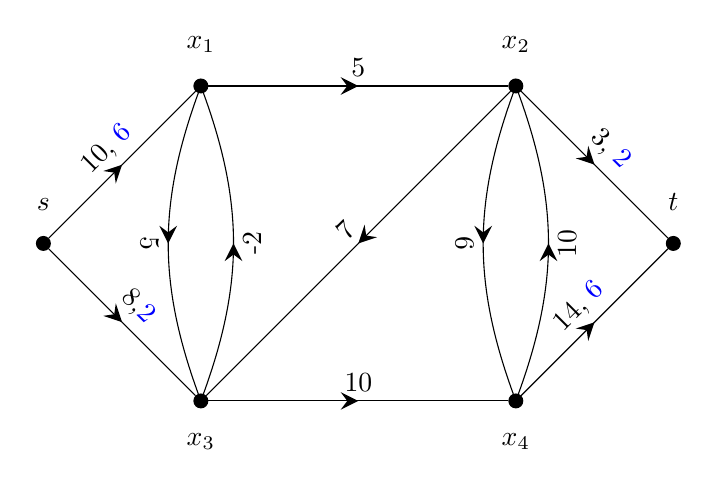
\begin{tikzpicture}[
    vertex/.style={circle, draw, fill=black, minimum size=5pt, inner sep=0pt},
    label distance=2mm  % 调整标签距离线的距离
]

  % 定义顶点位置
  \node[vertex, label=above:$x_1$] (x1) at (2,2) {};
  \node[vertex, label=below:$x_3$] (x3) at (2,-2) {};
  \node[vertex, label=above:$x_2$] (x2) at (6,2) {};
  \node[vertex, label=below:$x_4$] (x4) at (6, -2) {};
  \node[vertex, label=above:$s$] (s) at (0, 0) {};
  \node[vertex, label=above:$t$] (t) at (8, 0) {};

  % 绘制有向边并添加数字标签
  \draw[big arrow] (s) -- (x1) node[midway, above, sloped] {10, \textcolor{blue}{6}};
  \draw[big arrow] (s) -- (x3) node[midway, above, sloped] {8,\textcolor{blue}{2}};
  \draw[big arrow] (x2) -- (t) node[midway, above, sloped] {3, \textcolor{blue}{2}};
  \draw[big arrow] (x4) -- (t) node[midway, above, sloped] {14, \textcolor{blue}{6}};
  \draw[big arrow] (x1) -- (x2) node[midway, above, sloped] {5};
  \draw[big arrow] (x3) -- (x4) node[midway, above, sloped] {10};
  \draw[big arrow] (x2) -- (x3) node[midway, above, sloped] {7};
  
  \draw[big arrow] (x1) to [bend right=20] node[midway, below, sloped] {5} (x3);
  \draw[big arrow] (x3) to [bend right=20] node[midway, below, sloped] {-2} (x1);

  \draw[big arrow] (x2) to [bend right=20] node[midway, below, sloped] {6} (x4);
  \draw[big arrow] (x4) to [bend right=20] node[midway, below, sloped] {10} (x2);
\end{tikzpicture}

Flow $= 8$.
\end{example}

\setcounter{lemma}{3}
\begin{lemma}\label{lemma 3.4}
    Let $f$ be a flow of $(D, s, c,t)$. Then 
    \begin{align}
        \sum\limits_{y\in\Gamma^+(s)} f(sy) - \sum\limits_{z\in\Gamma^-(s)}f(zs) = \sum\limits_{z\in\Gamma^-(t)} f(zt) - \sum\limits_{y\in\Gamma^+(t)}f(ty) \label{3.3}
    \end{align}

   That is, net amount flowing out of $s = $net amount flowing into $t$. The \uline{\textcolor{MarkerColour}{\textsc{value}}} $v(f)$ of $f$ is the common value of \ref{3.3}. If particular, if $\Gamma^+(s) = \Gamma^+(t) = \varnothing$, then
   \begin{align*}
       \sum\limits_{y\in\Gamma^+(s)} f(sy) = \sum\limits_{z\in\Gamma^-(t)} f(zt)
   \end{align*}
\end{lemma}

\begin{proof}
    Note that 
    \begin{align*}
        \sum\limits_{v\in V(D)} \underbrace{\left( \sum\limits_{y\in\Gamma^+(x)} f(xy) - \sum\limits_{z\in\Gamma^-(x)}f(zx) \right) }\limits_{\color{red}{(*)}}= 0
    \end{align*}
    since at $x$, then terms $f(xy)$ and $-f(zx)$ are cancelled by the terms $-f(xy)$ and $f(zx)$ from $y$ and $z$. Thus \ref{3.2} $\Longrightarrow$ The terms $\color{red}{(*)} = 0$, except when $x = s,t$ and $\Longrightarrow$ \ref{3.3}
\end{proof}

By, lemma \ref{lemma 3.4}, we may ask:

\subsection{Problem 3.5} Given a flow network $(D, c, s, t)$, find a \uline{maximum flow}, that is, a flow $f$ s.t. $v(f)$ is maximum.

\subsubsection{Folk-Fulkerson Algorithm} 
\begin{definition}
    Given $(D, c, s, t)$, let $a_1, \cdots, a_k\in A(D)$ be s.t. when their directions are ignored, we have a graph path $x_0x_1\cdots x_k$, where $a_i = x_{i-1}x_i$ or $x_{i}x_{i-1}$, $\forall 1\leqslant i \leqslant k$. Assign a symbol $p_i/q_i$ to $a_i\ (1\leqslant i\leqslant k)$, where $p_i+q_i = c(a_i)$, and $p_i, q_i\geqslant 0$. The $a_i$ form an $x_0$-$x_k$ augmenting path if 
    \begin{align*}
        \left\lbrace\begin{array}{lll}
            p_i>0, &\ \text{if}\ a_i = x_{i-1}x_i: &\ a_i\ \text{is a \uline{forward arc}} \\
            q_i>0, &\ \text{if}\ a_i = x_{i}x_{i-1}: &\ a_i \text{is a \uline{backward arc}} 
        \end{array} \right.
    \end{align*}

    \tikzset{
    big arrow/.style={
        decoration={
            markings,
            mark=at position 0.5 with {\arrow[scale=2]{stealth}} % 调整这里的scale值来改变箭头大小
        },
        postaction={decorate}
    },
    vertex/.style={circle, draw, fill=black, minimum size=5pt, inner sep=0pt},
    label distance=2mm  % 调整标签距离线的距离
}

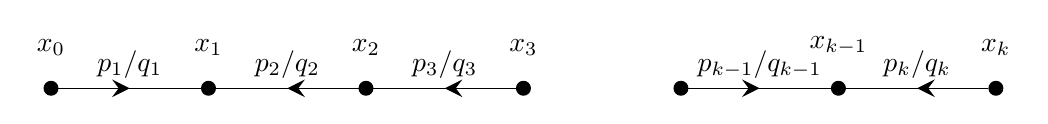
\begin{tikzpicture}[
    vertex/.style={circle, draw, fill=black, minimum size=5pt, inner sep=0pt},
    label distance=2mm  % 调整标签距离线的距离
]

  % 定义顶点位置
  \node[vertex, label=above:$x_0$] (x0) at (0,0) {};
  \node[vertex, label=above:$x_1$] (x1) at (2,0) {};
  \node[vertex, label=above:$x_2$] (x2) at (4,0) {};
  \node[vertex, label=above:$x_3$] (x3) at (6,0) {};
  \node[vertex, label=above:] (xk-2) at (8, 0) {};
  \node[vertex, label=above:$x_{k-1}$] (xk-1) at (10, 0) {};
  \node[vertex, label=above:$x_k$] (xk) at (12, 0) {};

  % 绘制有向边并添加数字标签
  \draw[big arrow] (x0) -- (x1) node[midway, above, sloped] {$p_1/q_1$};
  \draw[big arrow] (x2) -- (x1) node[midway, above, sloped] {$p_2/q_2$};
  \draw[big arrow] (x3) -- (x2) node[midway, above, sloped] {$p_3/q_3$};
  \draw[big arrow] (xk) -- (xk-1) node[midway, above, sloped] {$p_k/q_k$};
  \draw[big arrow] (xk-2) -- (xk-1) node[midway, above, sloped] {$p_{k-1}/q_{k-1}$};
\end{tikzpicture}
\end{definition}

The \uline{Ford-Fulkerson Algorithm} for solving Problem 3.5 is as follows.
\begin{itemize}
    \item Label the arcs of $D$ as $a_1, \cdots, a_m\ (m = |A(D)|)$. Assign $c(a_i)/0$ to $a_i$, $\forall 1\leqslant i\leqslant m$.
    \item Suppose $a_i$ is labelled with $p_i/q_i\ (1\leqslant i\leqslant m)$. Choose an $s$-$t$ augmenting with arcs $b_1, \cdots, b_k$, labelled with $p^{\prime}_i/q^{\prime}_i\ (1\leqslant i\leqslant k)$. Let 
    \begin{align*}
        r = \min \left(\min \{p_i^{\prime}:\ b_i\ \text{is forward}\},\ \min \{q_i^{\prime}:\ b_i\ \text{is backward}\}\right) > 0
    \end{align*}

    Update $p^{\prime}_i/q^{\prime}_i$ to
    \begin{align*}
        p^{\prime}_i/q^{\prime}_i = \left\lbrace\begin{array}{ll}
            p^{\prime}_i - r/q^{\prime}_i + r, &\ \text{if} \ b_i \ \text{is forward},  \\
            p^{\prime}_i + r/q^{\prime}_i - r, &\ \text{if} \ b_i \ \text{is backward}.
        \end{array} \right.
    \end{align*}

    This directs a flow of $r>0$ from $s$ to $t$ along the $s$-$t$ augmenting path.
    \item Repeat Step 2 until $\neg\exists\ s$-$t$ augmenting path. The maximum flow is the sum of all the $r$'s, achieved by the final $q_i$'s
\end{itemize}
\newcommand{\setexampletoVariant}[1]{%
    \setcounter{example}{#1}%
    \renewcommand{\theexample}{\arabic{example}$'$}%
}
\setexampletoVariant{2}

\begin{example}
    Again

    \tikzset{
    big arrow/.style={
        decoration={
            markings,
            mark=at position 0.5 with {\arrow[scale=2]{stealth}} % 调整这里的scale值来改变箭头大小
        },
        postaction={decorate}
    },
    vertex/.style={circle, draw, fill=black, minimum size=5pt, inner sep=0pt},
    label distance=2mm  % 调整标签距离线的距离
}

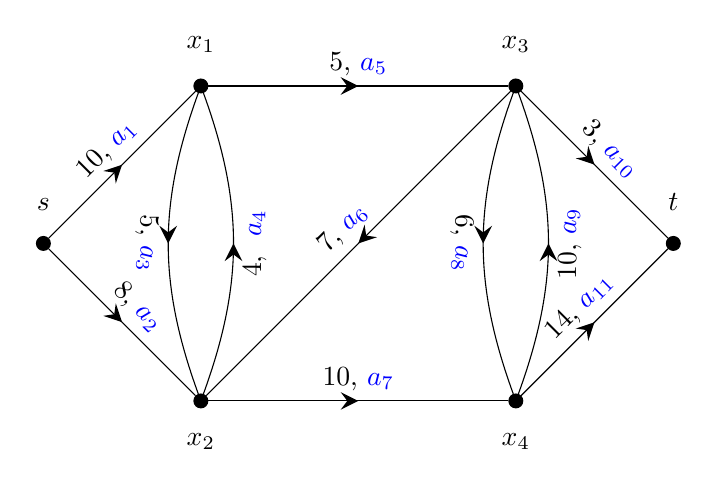
\begin{tikzpicture}[
    vertex/.style={circle, draw, fill=black, minimum size=5pt, inner sep=0pt},
    label distance=2mm  % 调整标签距离线的距离
]

  % 定义顶点位置
  \node[vertex, label=above:$x_1$] (x1) at (2,2) {};
  \node[vertex, label=below:$x_2$] (x3) at (2,-2) {};
  \node[vertex, label=above:$x_3$] (x2) at (6,2) {};
  \node[vertex, label=below:$x_4$] (x4) at (6, -2) {};
  \node[vertex, label=above:$s$] (s) at (0, 0) {};
  \node[vertex, label=above:$t$] (t) at (8, 0) {};

  % 绘制有向边并添加数字标签
  \draw[big arrow] (s) -- (x1) node[midway, above, sloped] {10,\ \textcolor{blue}{$a_1$}};
  \draw[big arrow] (s) -- (x3) node[midway, above, sloped] {8,\ \textcolor{blue}{$a_2$}};
  \draw[big arrow] (x2) -- (t) node[midway, above, sloped] {3, \textcolor{blue}{$a_{10}$}};
  \draw[big arrow] (x4) -- (t) node[midway, above, sloped] {14, \textcolor{blue}{$a_{11}$}};
  \draw[big arrow] (x1) -- (x2) node[midway, above, sloped] {5,\ \textcolor{blue}{$a_5$}};
  \draw[big arrow] (x3) -- (x4) node[midway, above, sloped] {10,\ \textcolor{blue}{$a_7$}};
  \draw[big arrow] (x2) -- (x3) node[midway, above, sloped] {7,\ \textcolor{blue}{$a_6$}};
  
  \draw[big arrow] (x1) to [bend right=20] node[midway, below, sloped] {5,\ \textcolor{blue}{$a_3$}} (x3);
  \draw[big arrow] (x3) to [bend right=20] node[midway, below, sloped] {4, \ \textcolor{blue}{$a_4$}} (x1);

  \draw[big arrow] (x2) to [bend right=20] node[midway, below, sloped] {6,\ \textcolor{blue}{$a_8$}} (x4);
  \draw[big arrow] (x4) to [bend right=20] node[midway, below, sloped] {10,\ \textcolor{blue}{$a_9$}} (x2);
\end{tikzpicture}
\end{example}

We proceed as follows.
\begin{table}[H]
    \centering
    \begin{tabular}{|ccccccccccc|c|c|}
        \hline
        $a_1$ & $a_2$ & $a_3$ & $a_4$ & $a_5$ & $a_6$ & $a_7$ & $a_8$ & $a_9$ & $a_{10}$ & $a_{11}$ & $s$-$t$ augmenting path & flow  \\ \hline
        \uline{10}/0 & 8/0 & 5/0 & 4/0 & \uline{5}/0 & 7/0 & 10/0 & 6/0 & 10/0 & \uline{3}/0 & 14/0 & $a_1 a_5 a_{10}$ & 3 \\
        7/3 & \uline{8}/0 & 5/0 & 4/0 & 2/3 & 7/0 & \uline{10}/0 & 6/0 & 10/0 & 0/3 & \uline{14}/0 & $a_2 a_7 a_{11}$ & 8 \\
        \uline{7}/3 & 0/8 & 5/0 & 4/0 & \uline{2}/3 & \uline{7}/0 & \uline{2}/8 & 6/0 & 2/8 & 0/3 & \uline{6}/8 & $a_1 a_5 a_6 a_7 a_{11}$ & 2 \\
        \uline{5}/5 & 0/8 & \uline{5}/0 & 4/0 & 0/5 & 5/\uline{2} & 0/10 & \uline{6}/0 & 2/8 & 0/3 & \uline{4}/10 & $a_1 a_3 \overleftarrow{a_6} a_8 a_{11}$ & 2 \\
        3/7 & 0/8 & 3/2 & 4/0 & 0/5 & 7/0 & 0/10 & 4/2 & 10/0 & 0/3 & 2/12 & & \\ \hline
    \end{tabular}
\end{table}

The bottom row has no $s$-$t$ augmenting path. The maximum flow is $3+8+2+2 = 15$, achieved as follows:

    \tikzset{
    big arrow/.style={
        decoration={
            markings,
            mark=at position 0.5 with {\arrow[scale=2]{stealth}} % 调整这里的scale值来改变箭头大小
        },
        postaction={decorate}
    },
    vertex/.style={circle, draw, fill=black, minimum size=5pt, inner sep=0pt},
    label distance=2mm  % 调整标签距离线的距离
}

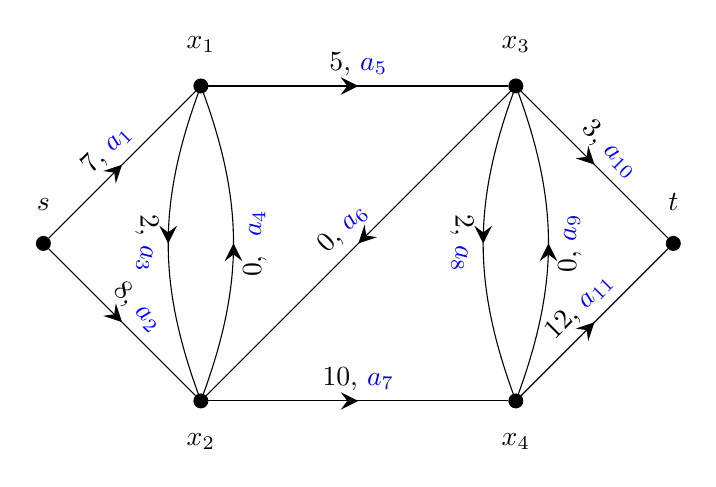
\begin{tikzpicture}[
    vertex/.style={circle, draw, fill=black, minimum size=5pt, inner sep=0pt},
    label distance=2mm  % 调整标签距离线的距离
]

  % 定义顶点位置
  \node[vertex, label=above:$x_1$] (x1) at (2,2) {};
  \node[vertex, label=below:$x_2$] (x3) at (2,-2) {};
  \node[vertex, label=above:$x_3$] (x2) at (6,2) {};
  \node[vertex, label=below:$x_4$] (x4) at (6, -2) {};
  \node[vertex, label=above:$s$] (s) at (0, 0) {};
  \node[vertex, label=above:$t$] (t) at (8, 0) {};

  % 绘制有向边并添加数字标签
  \draw[big arrow] (s) -- (x1) node[midway, above, sloped] {7,\ \textcolor{blue}{$a_1$}};
  \draw[big arrow] (s) -- (x3) node[midway, above, sloped] {8,\ \textcolor{blue}{$a_2$}};
  \draw[big arrow] (x2) -- (t) node[midway, above, sloped] {3, \textcolor{blue}{$a_{10}$}};
  \draw[big arrow] (x4) -- (t) node[midway, above, sloped] {12, \textcolor{blue}{$a_{11}$}};
  \draw[big arrow] (x1) -- (x2) node[midway, above, sloped] {5,\ \textcolor{blue}{$a_5$}};
  \draw[big arrow] (x3) -- (x4) node[midway, above, sloped] {10,\ \textcolor{blue}{$a_7$}};
  \draw[big arrow] (x2) -- (x3) node[midway, above, sloped] {0,\ \textcolor{blue}{$a_6$}};
  
  \draw[big arrow] (x1) to [bend right=20] node[midway, below, sloped] {2,\ \textcolor{blue}{$a_3$}} (x3);
  \draw[big arrow] (x3) to [bend right=20] node[midway, below, sloped] {0, \ \textcolor{blue}{$a_4$}} (x1);

  \draw[big arrow] (x2) to [bend right=20] node[midway, below, sloped] {2,\ \textcolor{blue}{$a_8$}} (x4);
  \draw[big arrow] (x4) to [bend right=20] node[midway, below, sloped] {0,\ \textcolor{blue}{$a_9$}} (x2);
\end{tikzpicture}

\begin{definition}
    Let $(D, c, s, t)$ be a flow network. For disjoint $X, Y\subset V(D)$, let
    \begin{align*}
        A(X, Y) &= \{xy\in A(D): x\in X, y\in Y\}, \\
        c(X, Y) &= \sum\limits_{xy\in A(X, Y)} c(xy) \\
    \end{align*}

    A \uline{\textcolor{MarkerColour}{\textsc{cut (separating $s$ and $t$}}} is a set $A(X, \bar{X})$, where $s\in X$, $t\in \bar{X}$ and $\bar{X} = V(D)\backslash X$. Thus by deleting a cut $A(X, \bar{X})$ from $D$, the remaining subdigraph $D^{\prime} = (V(D), A(D)\backslash A(X, \bar{X}))$ is s.t. $t$ is not reachable from $s$. A \uline{\textcolor{MarkerColour}{\textsc{minimum cut}}} of $(D, c, s, t)$ is a cut $A(X, \bar{X})$ s.t. $c(X, \bar{X})$ is minimum.
\end{definition}

\tikzset{
    big arrow/.style={
        decoration={
            markings,
            mark=at position 0.5 with {\arrow[scale=2]{stealth}} % 调整这里的scale值来改变箭头大小
        },
        postaction={decorate}
    },
    vertex/.style={circle, draw, fill=black, minimum size=5pt, inner sep=0pt},
    label distance=2mm  % 调整标签距离线的距离
}

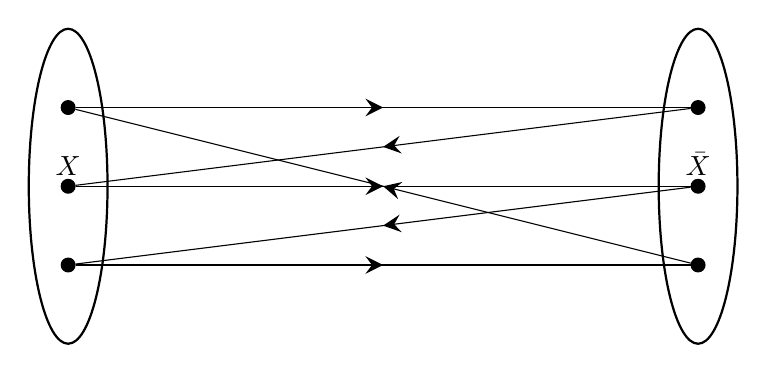
\begin{tikzpicture}[
    vertex/.style={circle, draw, fill=black, minimum size=5pt, inner sep=0pt},
    label distance=2mm  % 调整标签距离线的距离
]

% 绘制左侧的椭圆
\draw[thick] (-4, 0) ellipse (0.5 and 2) node[above] {$X$};;
% 左侧的点
\node[vertex] (A1) at (-4, 1) {};
\node[vertex] (A2) at (-4, 0) {};
\node[vertex] (A3) at (-4, -1) {};

% 绘制右侧的椭圆
\draw[thick] (4, 0) ellipse (0.5 and 2) node[above] {$\bar{X}$};
% 右侧的点
\node[vertex] (B1) at (4, 1) {};
\node[vertex] (B2) at (4, 0) {};
\node[vertex] (B3) at (4, -1) {};

% 绘制从左到右的连线
\draw[big arrow] (A1) -- (B1);
\draw[big arrow] (A2) -- (B2);
\draw[big arrow] (A3) -- (B3);

% 绘制从右到左的连线
\draw[big arrow] (B1) -- (A2);
\draw[big arrow] (B2) -- (A3);
\draw[big arrow] (B3) -- (A1);

% \node[anchor=west] at (7, 2) {$\longrightarrow \in A(X, \bar{X})$, $\longleftarrow \notin A(X, \bar{X})$}
\end{tikzpicture}

The Fold-Fulkersoon Algorithm also finds a minimum cut of $(D, c, s, t)$. When the algorithm terminates, let
\begin{align*}
    X = \{x\in V(D):\ \exists \ s-x\ \text{augmenting path w.r.t. final flow}\}\cup\{s\}
\end{align*}

Note that $t\in\bar{X}$, otherwise $\exists$ $s$-$t$ augmenting path when the algorithm terminated, a contradiction. So $A(X, \bar{X})$ is a cut, and in fact, a minimum cut.

\setcounter{example}{2}
\begin{example}
    After the algorithm terminates in Example 3', we see that $\exists$ $s$-$t$ augmenting path $\Longleftrightarrow$\ $x \in\{x_1, x_2\}$.
\end{example}

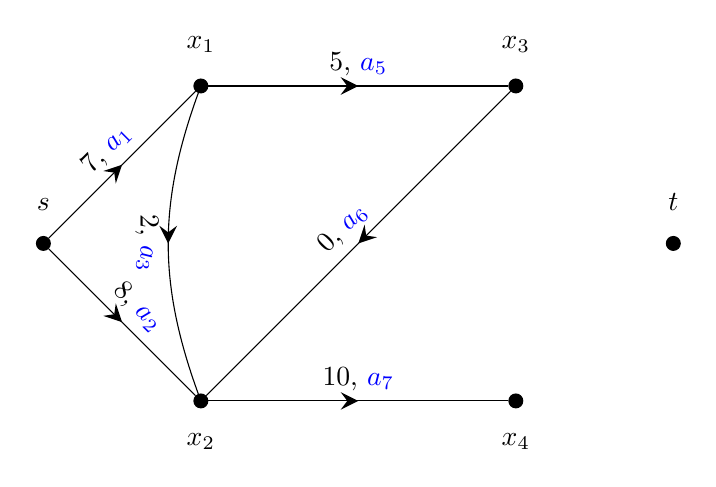
\begin{tikzpicture}[
    vertex/.style={circle, draw, fill=black, minimum size=5pt, inner sep=0pt},
    label distance=2mm  % 调整标签距离线的距离
]

  % 定义顶点位置
  \node[vertex, label=above:$x_1$] (x1) at (2,2) {};
  \node[vertex, label=below:$x_2$] (x3) at (2,-2) {};
  \node[vertex, label=above:$x_3$] (x2) at (6,2) {};
  \node[vertex, label=below:$x_4$] (x4) at (6, -2) {};
  \node[vertex, label=above:$s$] (s) at (0, 0) {};
  \node[vertex, label=above:$t$] (t) at (8, 0) {};

  % 绘制有向边并添加数字标签
  \draw[big arrow] (s) -- (x1) node[midway, above, sloped] {7,\ \textcolor{blue}{$a_1$}};
  \draw[big arrow] (s) -- (x3) node[midway, above, sloped] {8,\ \textcolor{blue}{$a_2$}};
  \draw[big arrow] (x1) -- (x2) node[midway, above, sloped] {5,\ \textcolor{blue}{$a_5$}};
  \draw[big arrow] (x3) -- (x4) node[midway, above, sloped] {10,\ \textcolor{blue}{$a_7$}};
  \draw[big arrow] (x2) -- (x3) node[midway, above, sloped] {0,\ \textcolor{blue}{$a_6$}};
  
  \draw[big arrow] (x1) to [bend right=20] node[midway, below, sloped] {2,\ \textcolor{blue}{$a_3$}} (x3);
\end{tikzpicture}

We have $X = \{s, x_1, x_2\}$, $\bar{X} = \{t, x_3, x_4\}$, and $A(X, \bar{X}) = \{a_5, a_7\}$ with $c(X, \bar{X}) = 5+10 = 15$.

We have the following result
\setcounter{theorem}{5}
\begin{theorem}[Max-flow min-cut Theorem]
    For a flow network $(D, c, s, t)$, the maximum flow is equal to $c(X, \bar{X})$, where $A(X, \bar{X})$ is a minimum cut.
\end{theorem}

We first prove:
\begin{theorem}[Flow value lemma]
    Let $f$ be a flow and $A(X, \bar{X})$ be a cut of $(D, c, s, t)$. Then 
    \begin{align*}
        v(f) = \sum\limits_{xy\in A(X, \bar{X})} f(xy) - \sum\limits_{yx\in A(\overline{X}, X)} f(yx) 
    \end{align*}
\end{theorem}

\begin{proof}
    We have 
    \begin{align*}
        v(f) &= \sum\limits_{y\in \Gamma^+(s)} f(sy) - \sum\limits_{z\in \Gamma^-_(s)} f(zs) \\
        &= \sum\limits_{x\in X} \underbrace{\left(\sum\limits_{y\in \Gamma^+(s)} f(xy) - \sum\limits_{z\in \Gamma^-_(s) } f(zx) \right)}\limits_{(*)},\ \text{the terms}\ (*) = 0,\ \text{except for}\ x=s \\
        &= \sum\limits_{xy\in A(X, \bar{X})} f(xy) - \sum\limits_{yx\in A(X, \bar{X})} f(yx), \ \text{arcs within}\ X \ \text{cancel}.
    \end{align*}
\end{proof}

\begin{proof}
    of Th 3.6. For any flow $g$ and any cut $A(Y, \bar{Y})$, we have $v(g)\leqslant c(Y, \bar{Y})$(HW5). So $v = \sup\{v(g):\ g\ \text{is a flow of}\ (D, c, s, t)\} < \infty$. We may take a sequence of flow $g_j: A(D)\to\mathbb{R}_{\geqslant 0}$ s.t. $v(g_j)\to v$ and $g_j(xy) \to f(xy)$, $\forall xy\in A(D)$ ($f$ is the point-wise limit of the $g_j$). Then $f$ is a minimum flow. Now, we construct a cut $A(X, \bar{X})$ s.t. $v(f) = c(X, \bar{X})$. Define 
    \begin{align*}
        X = \{ x\in V(D): \exists \ s-x\ \text{augmenting path w.r.t.}\ f\}\cup \{s\}
    \end{align*}

    We claim that $A(X, \bar{X})$ is a cut. Otherwise, suppose $t\in X$. Then $\exists s= x_0, x_1, \cdots, x_k = t \in V(D)$ s.t.
    \begin{align*}
        r_i = c(x_{i-1}x_i) - f(x_{i-1}x_i)\  \text{or} \ r_i = f(x_ix_{i-1})
    \end{align*}
    satisfies $r_i>0$, $\forall 1\leqslant i\leqslant k$. Let $r = \min\limits_i r_i >0$. We define the flow $f^*$ by 
    \begin{align*}
    \begin{array}{ll}
        f^*(x_{i-1}x_i) = f(x_{i-1}x_i) + r \leqslant c(x_{i-1}x_i),& \ \text{if}\ r_i = c(x_{i-1}x_i) - f(x_{i-1}x_i) \\
        f^*(x_{i-1}x_i) = f(x_i x_{i-1}) - r \geqslant 0,& \ \text{if} r_i = f(x_ix_{i-1}), \\
        f^*(a) = f(a), &\forall\ \text{other arcs}\ a.
    \end{array}
    \end{align*}

    Then $f^*$ is also a flow, and $v(f^*) = v(f) + r$ since either $sx_1$ increased by $r$, or $x_1 s$ decreased by $r$. This contradicts that $f$ is a maximum flow.

    Now, 
    \begin{align*}
        v(f) = \underset{=}{\text{Th 3.7}} \sum\limits_{xy\in A(X, \bar{X})} \underbrace{f(xy)}\limits_{= c(xy)} - \sum\limits_{yx\in A(X, \bar{X}} \underbrace{f(yx)}\limits_{=0} = c(X, \bar{X}),
    \end{align*}
    as required.
\end{proof}


\begin{theorem}
    The Ford-Fulkerson Algorithm, \uline{If} it terminates, solves Problem 3.5 for $(D,\ c,\ s,\ t)$ and also finds a minimum cut. Precisely, let $f$ be the final flow, and 
    \begin{align*}
        X = \{x\in V(D):\ \exists\ s-x\ \text{augmenting path w.r.t}\ f\} \cup \{s\}
    \end{align*}

    Then $f$ is a maximum flow, and $A(X,\ \overline{X})$ is a minimum cut.
\end{theorem}
\begin{proof}
    From the discussion before Example 3'', $A(X,\ \overline{X})$ is a cut. Note that if $xy\in A(X,\ \overline{X})$ then $f(xy) = c(xy)$, and if $yx\in A(X,\ \overline{X})$ then $f(yx) = 0$. Otherwise, in either case, $\exists\ s-y$ augmenting path: Take an $s-x$ augmenting path, which must be within $X$, then go along $xy$ or $yx$ to $y$. Thus
    \begin{align*}
        v(f) = \underset{L\ 3.7}{=} \sum\limits_{xy\in A(X,\overline{X})} \underbrace{f(xy)}\limits_{=c(xy)} - \sum\limits_{yx\in A(\overline{X},X)} \underbrace{f(yx)}\limits_{=0} = c(X,\overline{X})
    \end{align*}

    If $A(Y,\ \overline{Y})$ is a minimum cut, then $c(X,\ \overline{X}) = v(f) \leqslant c(Y,\ \overline{Y})$ (HW5). So $A(X,\ \overline{X})$ is a minimum cut, and Th 3.6 $\Rightarrow\ f$ is a maximum flow. 
\end{proof}

\begin{remark}
    The Fold-Fulkersoon Algorithm terminates if $c:\ A(D)\to\mathbb{Z}_{\geqslant 0}$, since each iteration increase the currently known flow by $\geqslant 1$. The algorithm also terminates if $c:\ A(D)\to\mathbb{Q}_{\geqslant 0}$, since we may consider $c^{\prime}:A(D)\to\mathbb{Z}_{\geqslant 0}$ by multiplying the denominators of $c(xy)$, $\forall\ xy\in A(D)$ by a common multiple. But the algorithm may possible not terminate if $c:A(D)\to\mathbb{R}_{\geqslant 0}$. For example:
    
    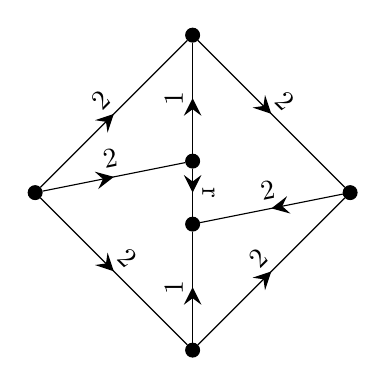
\begin{tikzpicture}[
    vertex/.style={circle, draw, fill=black, minimum size=5pt, inner sep=0pt},
    label distance=2mm  % 调整标签距离线的距离
]

  % 定义顶点位置
  \node[vertex] (x1) at (0,2) {};
  \node[vertex] (x2) at (-2,0) {};
  \node[vertex] (x3) at (2,0) {};
  \node[vertex] (x4) at (0, -2) {};
  \node[vertex] (x5) at (0, 0.4) {};
  \node[vertex] (x6) at (0, -0.4) {};

  % 绘制有向边并添加数字标签
  \draw[big arrow] (x2) -- (x1) node[midway, above, sloped] {2};
  \draw[big arrow] (x1) -- (x3) node[midway, above, sloped] {2};
  \draw[big arrow] (x2) -- (x4) node[midway, above, sloped] {2};
  \draw[big arrow] (x4) -- (x3) node[midway, above, sloped] {2};
  \draw[big arrow] (x2) -- (x5) node[midway, above, sloped] {2};
  \draw[big arrow] (x3) -- (x6) node[midway, above, sloped] {2};
  
  \draw[big arrow] (x5) -- (x1) node[midway, above, sloped] {1};
  \draw[big arrow] (x4) -- (x6) node[midway, above, sloped] {1};
  \draw[big arrow] (x5) -- (x6) node[midway, above, sloped] {r};
  
\end{tikzpicture}

$r = \frac{\sqrt{5}-1}{2}$, which satisfies $r^2 = 1-r$.
\end{remark}

\section{Minimum Spanning Tree Problem}
\begin{definition}
    A \uline{(connected) component} of a graph $G$ is a ``maximal connected subgraph'' $H\subset G$ in the following sense: $H$ is connected, and $\neg\exists\ xy\in E(G)\backslash E(H)$ s.t. $H^{\prime} = (V(H)\cup\{x,\ y\},\ E(H)\cup\{xy\})$ is connected.
\end{definition}

%%% G
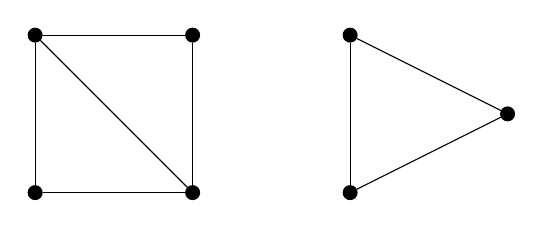
\begin{tikzpicture}[
    vertex/.style={circle, draw, fill=black, minimum size=5pt, inner sep=0pt},
    label distance=2mm  % 调整标签距离线的距离
]

  % 定义顶点位置
  \node[vertex] (x1) at (0,1) {};
  \node[vertex] (x2) at (0,-1) {};
  \node[vertex] (x3) at (2,1) {};
  \node[vertex] (x4) at (2,-1) {};
  \node[vertex] (x5) at (4, 1) {};
  \node[vertex] (x6) at (4, -1) {};
  \node[vertex] (x7) at (6, 0) {};
%  \node[vertex] (x8) at (8, 1) {};
  

  % 绘制有向边并添加数字标签
  \draw[-] (x1) -- (x2);
  \draw[-] (x2) -- (x4);
  \draw[-] (x3) -- (x4);
  \draw[-] (x4) -- (x1);
  \draw[-] (x1) -- (x3);

  \draw[-] (x5) -- (x6);
  \draw[-] (x6) -- (x7);
  \draw[-] (x7) -- (x5);
  
\end{tikzpicture}

A graph $T$ is a tree if $T$is connected; and does not contain q cycle as q subgraph. A graph $F$ is a forest if all components of $F$ are trees. A leaf of a graph is a vertex with degree $1$. Trees, with leaves circled.

\tikzset{every picture/.style={line width=0.75pt}} %set default line width to 0.75pt        

\begin{tikzpicture}[x=0.75pt,y=0.75pt,yscale=-1,xscale=1]
%uncomment if require: \path (0,300); %set diagram left start at 0, and has height of 300

%Straight Lines [id:da8778746157310466] 
\draw    (26.52,180.52) -- (53.81,102.84) -- (99.99,170.51) -- (153.11,106.6) -- (191.04,178.21) -- (236.56,112.35) ;
%Straight Lines [id:da982602405019146] 
\draw    (311.33,94.55) -- (315.4,146.07) -- (361.03,109.46) ;
%Straight Lines [id:da10558162526255566] 
\draw    (315.4,146.07) -- (340.36,179.43) ;
%Straight Lines [id:da9652131386469209] 
\draw    (281.55,176.92) -- (315.4,146.07) ;
%Straight Lines [id:da9098976808427328] 
\draw    (277.55,129.99) -- (315.4,146.07) ;
%Straight Lines [id:da6871756317261613] 
\draw    (458.32,75.75) -- (477.12,97.08) -- (501.63,75.98) ;
%Straight Lines [id:da8528625774476026] 
\draw    (471.01,123.31) -- (477.12,97.08) ;
%Straight Lines [id:da38370950515203894] 
\draw    (505.75,119.91) -- (471.01,123.31) ;
%Straight Lines [id:da11776512824599861] 
\draw    (442.15,144.6) -- (471.01,123.31) ;
%Straight Lines [id:da3101455899284844] 
\draw    (415.7,124.08) -- (442.15,144.6) ;
%Straight Lines [id:da7053915994545827] 
\draw    (507.92,168.38) -- (475.72,173.41) -- (442.15,144.6) ;
%Straight Lines [id:da6541004127841545] 
\draw    (487.63,201.13) -- (475.72,173.41) ;
%Straight Lines [id:da08969264363324325] 
\draw    (428.07,175.9) -- (442.15,144.6) ;
\end{tikzpicture}

\subsection{Problem 3.9 (Minimum Spanning Tree Problem)}
Let $(G, W)$ be a network graph, where $G$ is connected and $w:\ E(G)\to\mathbb{R}$. Find a \uline{minimum spanning tree (MST)}, that is, a spanning tree (ST) $T$ of $G$ s.t. $\sum\limits_{e\in E(T)} w(e)$ is minimum.

\uline{Kruskal's Algorithm} can solve Problem 3.9, and is as follows.

\paragraph{Kruskal's Algorithm}
\begin{itemize}
    \item Choose an edge $e_1\in E(G)$ with $w(e_i)$ minimum.
    \item Suppose edges $e_1,\cdots, e_k\in E(G)$ have been chosen, for some $k\geqslant 1$. Choose $e_{k+1}\in E(G)\backslash\{e_1,\cdots, e_k\}$ s.t. $e_{k+1}$ does not from a cycle with some of $e_1,\cdots, e_k$ and $w(e_{k+1})$ is minimum.
    \item Continue until $|V(G)| - 1$ edges are found. The result is a MST.
\end{itemize}

\setcounter{example}{3}
\begin{example}
    Let $(G, W)$ be

    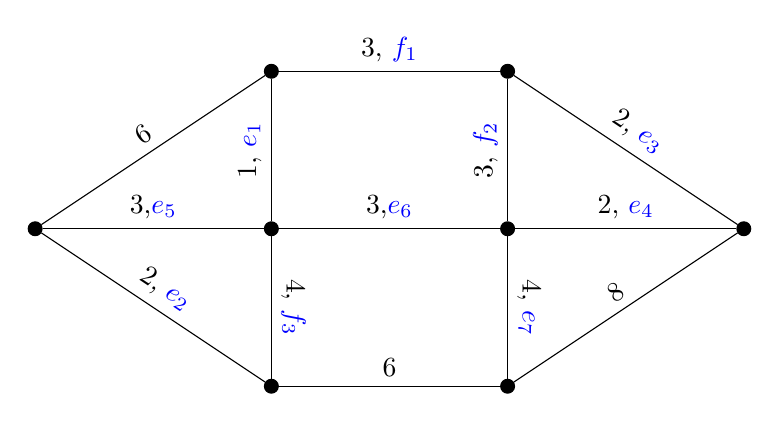
\begin{tikzpicture}[
    vertex/.style={circle, draw, fill=black, minimum size=5pt, inner sep=0pt},
    label distance=1mm  % 调整标签距离线的距离
]

  % 定义顶点位置
  \node[vertex] (x1) at (0,0) {};
  \node[vertex] (x2) at (3,2) {};
  \node[vertex] (x3) at (3,-2) {};
  \node[vertex] (x) at (3,0) {};
  \node[vertex] (y) at (6,0) {};
  \node[vertex] (x4) at (6, 2) {};
  \node[vertex] (x5) at (6, -2) {};
  \node[vertex] (x6) at (9, 0) {};

  % 绘制有向边并添加数字标签
  \draw[-] (x1) -- (x2) node[midway, above, sloped] {6};
  \draw[-] (x1) -- (x3) node[midway, above, sloped] {2, \textcolor{blue}{$e_2$}};
  \draw[-] (x1) -- (x) node[midway, above, sloped] {3,\textcolor{blue}{$e_5$}};
  \draw[-] (x) -- (y) node[midway, above, sloped] {3,\textcolor{blue}{$e_6$}};
  \draw[-] (x) -- (x2) node[midway, above, sloped] {1, \textcolor{blue}{$e_1$}};
  \draw[-] (x) -- (x3) node[midway, above, sloped] {4, \textcolor{blue}{$f_3$}};
  \draw[-] (x2) -- (x4) node[midway, above, sloped] {3, \textcolor{blue}{$f_1$}};
  \draw[-] (x4) -- (x6) node[midway, above, sloped] {2, \textcolor{blue}{$e_3$}};
  \draw[-] (y) -- (x6) node[midway, above, sloped] {2, \textcolor{blue}{$e_4$}};
  
  \draw[-] (y) -- (x4) node[midway, above, sloped] {3, \textcolor{blue}{$f_2$}};
  \draw[-] (x5) -- (x6) node[midway, above, sloped] {8};
  \draw[-] (x3) -- (x5) node[midway, above, sloped] {6};

  \draw[-] (y) -- (x5) node[midway, above, sloped] {4, \textcolor{blue}{$e_7$}};
\end{tikzpicture}
\end{example}

We ``greedily'' choose $e_1,\cdots, e_6$, since they have the smallest weights, and do not from a cycle. Then we cannot choose $f_1$ or $f_2$ since adding either edge forms a cycle. We can then choose $e_7$ (but not $f_3$) to obtain the MST. The weight is $1+2+2+2+3+3+4 = 17$.
    
\begin{tikzpicture}[
    vertex/.style={circle, draw, fill=black, minimum size=5pt, inner sep=0pt},
    label distance=1mm  % 调整标签距离线的距离
]

  % 定义顶点位置
  \node[vertex] (x1) at (0,0) {};
  \node[vertex] (x2) at (3,2) {};
  \node[vertex] (x3) at (3,-2) {};
  \node[vertex] (x) at (3,0) {};
  \node[vertex] (y) at (6,0) {};
  \node[vertex] (x4) at (6, 2) {};
  \node[vertex] (x5) at (6, -2) {};
  \node[vertex] (x6) at (9, 0) {};

  % 绘制有向边并添加数字标签
  \draw[-] (x1) -- (x3) node[midway, above, sloped] {2, \textcolor{blue}{$e_2$}};
  \draw[-] (x1) -- (x) node[midway, above, sloped] {3,\textcolor{blue}{$e_5$}};
  \draw[-] (x) -- (y) node[midway, above, sloped] {3,\textcolor{blue}{$e_6$}};
  \draw[-] (x) -- (x2) node[midway, above, sloped] {1, \textcolor{blue}{$e_1$}};
  \draw[-] (x4) -- (x6) node[midway, above, sloped] {2, \textcolor{blue}{$e_3$}};
  \draw[-] (y) -- (x6) node[midway, above, sloped] {2, \textcolor{blue}{$e_4$}};
  \draw[-] (y) -- (x5) node[midway, above, sloped] {4, \textcolor{blue}{$e_7$}};
\end{tikzpicture}

\begin{theorem}
    Kruskal's Algorithm solves Problem 3.9.
\end{theorem}
\begin{proof}
    Let $|V(G)| = n$. We first show that when the algorithm terminates, we have a $ST$ $T$ of $G$. 

    Initially, we have a forest with $n$ single vertices as components. Suppose that after $t$ iterations $(0\leqslant t\leqslant n-2)$, the current graph $F$ is a forest with $n-t$ components. If we add a new edge $xy$ to $F$ to form $F^+$, then we cannot have $x, y$ belonging to the same component of $F$, otherwise we create a cycle. Also, since $G$ is connected, we may add $xy$ where $x, y$ belong to two different components $F_1, F_2$ of $F$. The new component $F^{\prime} = \left(V(F_1)\cup V(F_2),\ E(F_1)\cup E(F_2) \cup\{xy\} \right)$ of $F^+$ is also a tree. Clearly $F^{\prime}$ is connected, and if $\exists$ cycle $C\subset F^{\prime}$, then $\exists\ e, e^{\prime}\in E(C)$, each one connecting $F_1$ and $F_2$, a contradiction since $xy$ is the only such edge in $F^{\prime}$. Thus, $F^+$ is a forest with $n-t-1$ components. Iterating $n-1$ times gives a ST T of G.

    Now, we prove that $T$ is a MST. Let $e_1,\cdots, e_{n-1}$ chosen in that order, so $w(e_1)\leqslant\cdots\leqslant w(e_{n-1})$. If $T$ is not a MST, choose a MST $S\subset G$ s.t. $|E(S)\cap E(T)|$ is maximum. Let $1\leqslant k \leqslant n-1$ be s.t. $e_1,\cdots, e_{k-1}\in E(S)\cap E(T)$, and $e_k\in E(T)\backslash E(S)$. Then $S^{\prime} = (V(S), E(S)\cup\{e_k\})$ has a cycle $C^{\prime}$. Now, $\exists\ f\in E(C^{\prime})\backslash E(T)$. Then $S^{\prime\prime} = (V(S^{\prime},\ E(S^{\prime})\backslash\{f\})$ is also a ST, since $S^{\prime\prime}$ is connected and has $n-1$ edges (HW6). To see that $S^{\prime\prime}$ is connected, let $u,\ v\in V(S^{\prime\prime}$. Then $\exists\ u-v$ path $P\subset S^{\prime}$. Either $P\subset S^{\prime\prime}$, or $f\in E(P)$. If the latter, let $f= zz^{\prime}$. Then $\exists\ u-z$ and $z^{\prime}-v$ paths $\subset P$, and a $z-z^{\prime}$ path in $C^{\prime}$, not using $f$. These paths $\Longrightarrow$ $\exists\ u-v$ path in $S^{\prime\prime}$. 

    Now $\sum\limits_{e\in E(S^{\prime\prime})} w(e) \geqslant \sum\limits_{e\in E(S)} w(e)\ \Longrightarrow\ w(e_k)\geqslant w(f)$. Since $e_1,\cdots, e_{k-1}, e_k\in E(T)$ and $e_1,\cdots, e_{k-1},f\in E(S)$, neither of these sets of edges creates a cycle, and since the algorithm chose $e_k$ instead of $f$, we have $w(e_k)\geqslant w(f)$. So $w(e_k)=w(f)$, and $S^{\prime\prime}$ is also a MST. But then $|E(S^{\prime\prime})\cap E(T)| = |E(S)\cap E(T)| + 1$, which contradicts the choice of $S$.
\end{proof}

\begin{remark}
    \begin{itemize}
        \item Kruskal's Algorithm also work if some edges of $G$ has negative weights.
        \item If these is a tie for the choice of edges with minimum weight at an iteration, we may choose any suitable edge.
        \item If $G$ has $q$ components, then Kruskal's Algorithm finds a minimum spanning forest in $n-q$ iterations.
    \end{itemize}
\end{remark}

\setcounter{proposition}{10}
\begin{proposition}
    Let $T$ be a tree with $n\geqslant 2$ vertices. 
    \begin{itemize}
        \item[(a)] $T$ has a leaf.
        \item[(b)] Deleting a leaf $x$ and the edge $e$ incident to $x$ from $T$ gives another tree $T^{\prime}$.
    \end{itemize}
\end{proposition}
\begin{proof}
    True for $n=2$. Assume $n\geqslant 3$.
    \begin{itemize}
        \item[(a)] Let $P = x_0 x_1\cdots x_k\subset T$ be a longest path, for some $k\geqslant 2$. Then $\Gamma(x_k)\subset\{x_0,\cdots,x_{k-1}\}$, otherwise we have a path longer than $P$. Also, $x_kx_i\notin E(T)$, $\forall 0\leqslant i\leqslant k-2$, otherwise $T$ has a cycle. So $\Gamma(x_k) = x_{k-1}$, and $x_k$ is a leaf.
        \item[(b)] Clearly $\neq\exists$ cycle in $T\Longrightarrow\ \neq\exists$ cycle in $T^{\prime}$. Let $u,v\in V(T^{\prime}) = V(T)\backslash\{x\}$. Then $\exists u-v$ path $Q\subset T$, and $Q$ cannot use $e$ and $x$ since $d(x)= 1$ in $T$. So $G\subset T^{\prime}$ and $T^{\prime}$ is connected.
    \end{itemize}
\end{proof}

Prop 3.11 is very useful for induction proofs involving trees.

